%%%%%%%%%%%%%%%%%%%%%%%%%%%%%%%%%%%%%%%%%
% NQCC Visit Presentation
% Based on the Imperial College London Beamer Template
%
%!TEX program = xelatex
% Note: this must be compiled with XeLaTeX (not pdfLaTeX) due to the custom fonts.
%%%%%%%%%%%%%%%%%%%%%%%%%%%%%%%%%%%%%%%%%

%----------------------------------------------------------------------------------------
%	CLASS, PACKAGES AND OTHER DOCUMENT CONFIGURATIONS
%----------------------------------------------------------------------------------------

\documentclass[
	aspectratio=169, % 16:9 aspect ratio
	t, % Top align all slide content by default
	onlytextwidth, % Typeset content in columns at text width
	10pt,
]{beamer}

\usetheme{Imperial}

%----------------------------------------------------------------------------------------
%	PRESENTATION INFORMATION
%----------------------------------------------------------------------------------------

\title{Atoms and Molecules in Tweezers}
\subtitle{State of the Experiment}
\author{Thomas Walker}
\date{\today}

%----------------------------------------------------------------------------------------

\begin{document}

%----------------------------------------------------------------------------------------
%	TITLE SLIDE
%----------------------------------------------------------------------------------------

\begingroup
	\setbeamercolor{background canvas}{bg=ICLBlue}
	\setbeamercolor{title page title}{fg=white}
	\setbeamercolor{title page subtitle}{fg=white}
	\setbeamercolor{author}{fg=white}
	\setbeamercolor{date}{fg=white}
	\setbeamertemplate{title page}[logo]{ICL_Logo_White.pdf}
	\frame[plain, s]{\titlepage}
\endgroup


\begingroup
	\setbeamercolor{background canvas}{bg=ICLBlue}
	\setbeamercolor{normal text}{fg=white}\usebeamercolor[fg]{normal text}
	\setbeamercolor{page number in head/foot}{fg=white}

	\begin{frame}
		{\Huge\textcolor{white}{{\ImperialSansSemiBold The Chamber(s)}}}
	\end{frame}
\endgroup

%------------------------------------------------

\begin{frame}
	\frametitle{Trapping CaF Molecules}

	\begin{columns}[T]
		\begin{column}{0.42\linewidth}
			\small
			\begin{itemize}
				\item CaF blue MOT \textasciitilde 2.5 - 3.0 $\times$ 10\textsuperscript{4} molecules at \textasciitilde 60 uK.
				\item Optical pumping, magnetic trapping of CaF and transport to the tweezer chamber.
				\item Transfer into a blue MOT in the tweezer chamber.
				\item Load CaF into 852 nm tweezer array from blue MOT.
			\end{itemize}

			\vspace{6pt}
			\textbf{Rydberg Excitation}
			\begin{itemize}
				\item \textbf{780 nm + 480 nm} - two-photon Rydberg excitation to 60s.
				\item \textbf{297 nm} - direct single-photon Rydberg excitation to 59p.
			\end{itemize}
		\end{column}
		\begin{column}{0.56\linewidth}
			\centering
			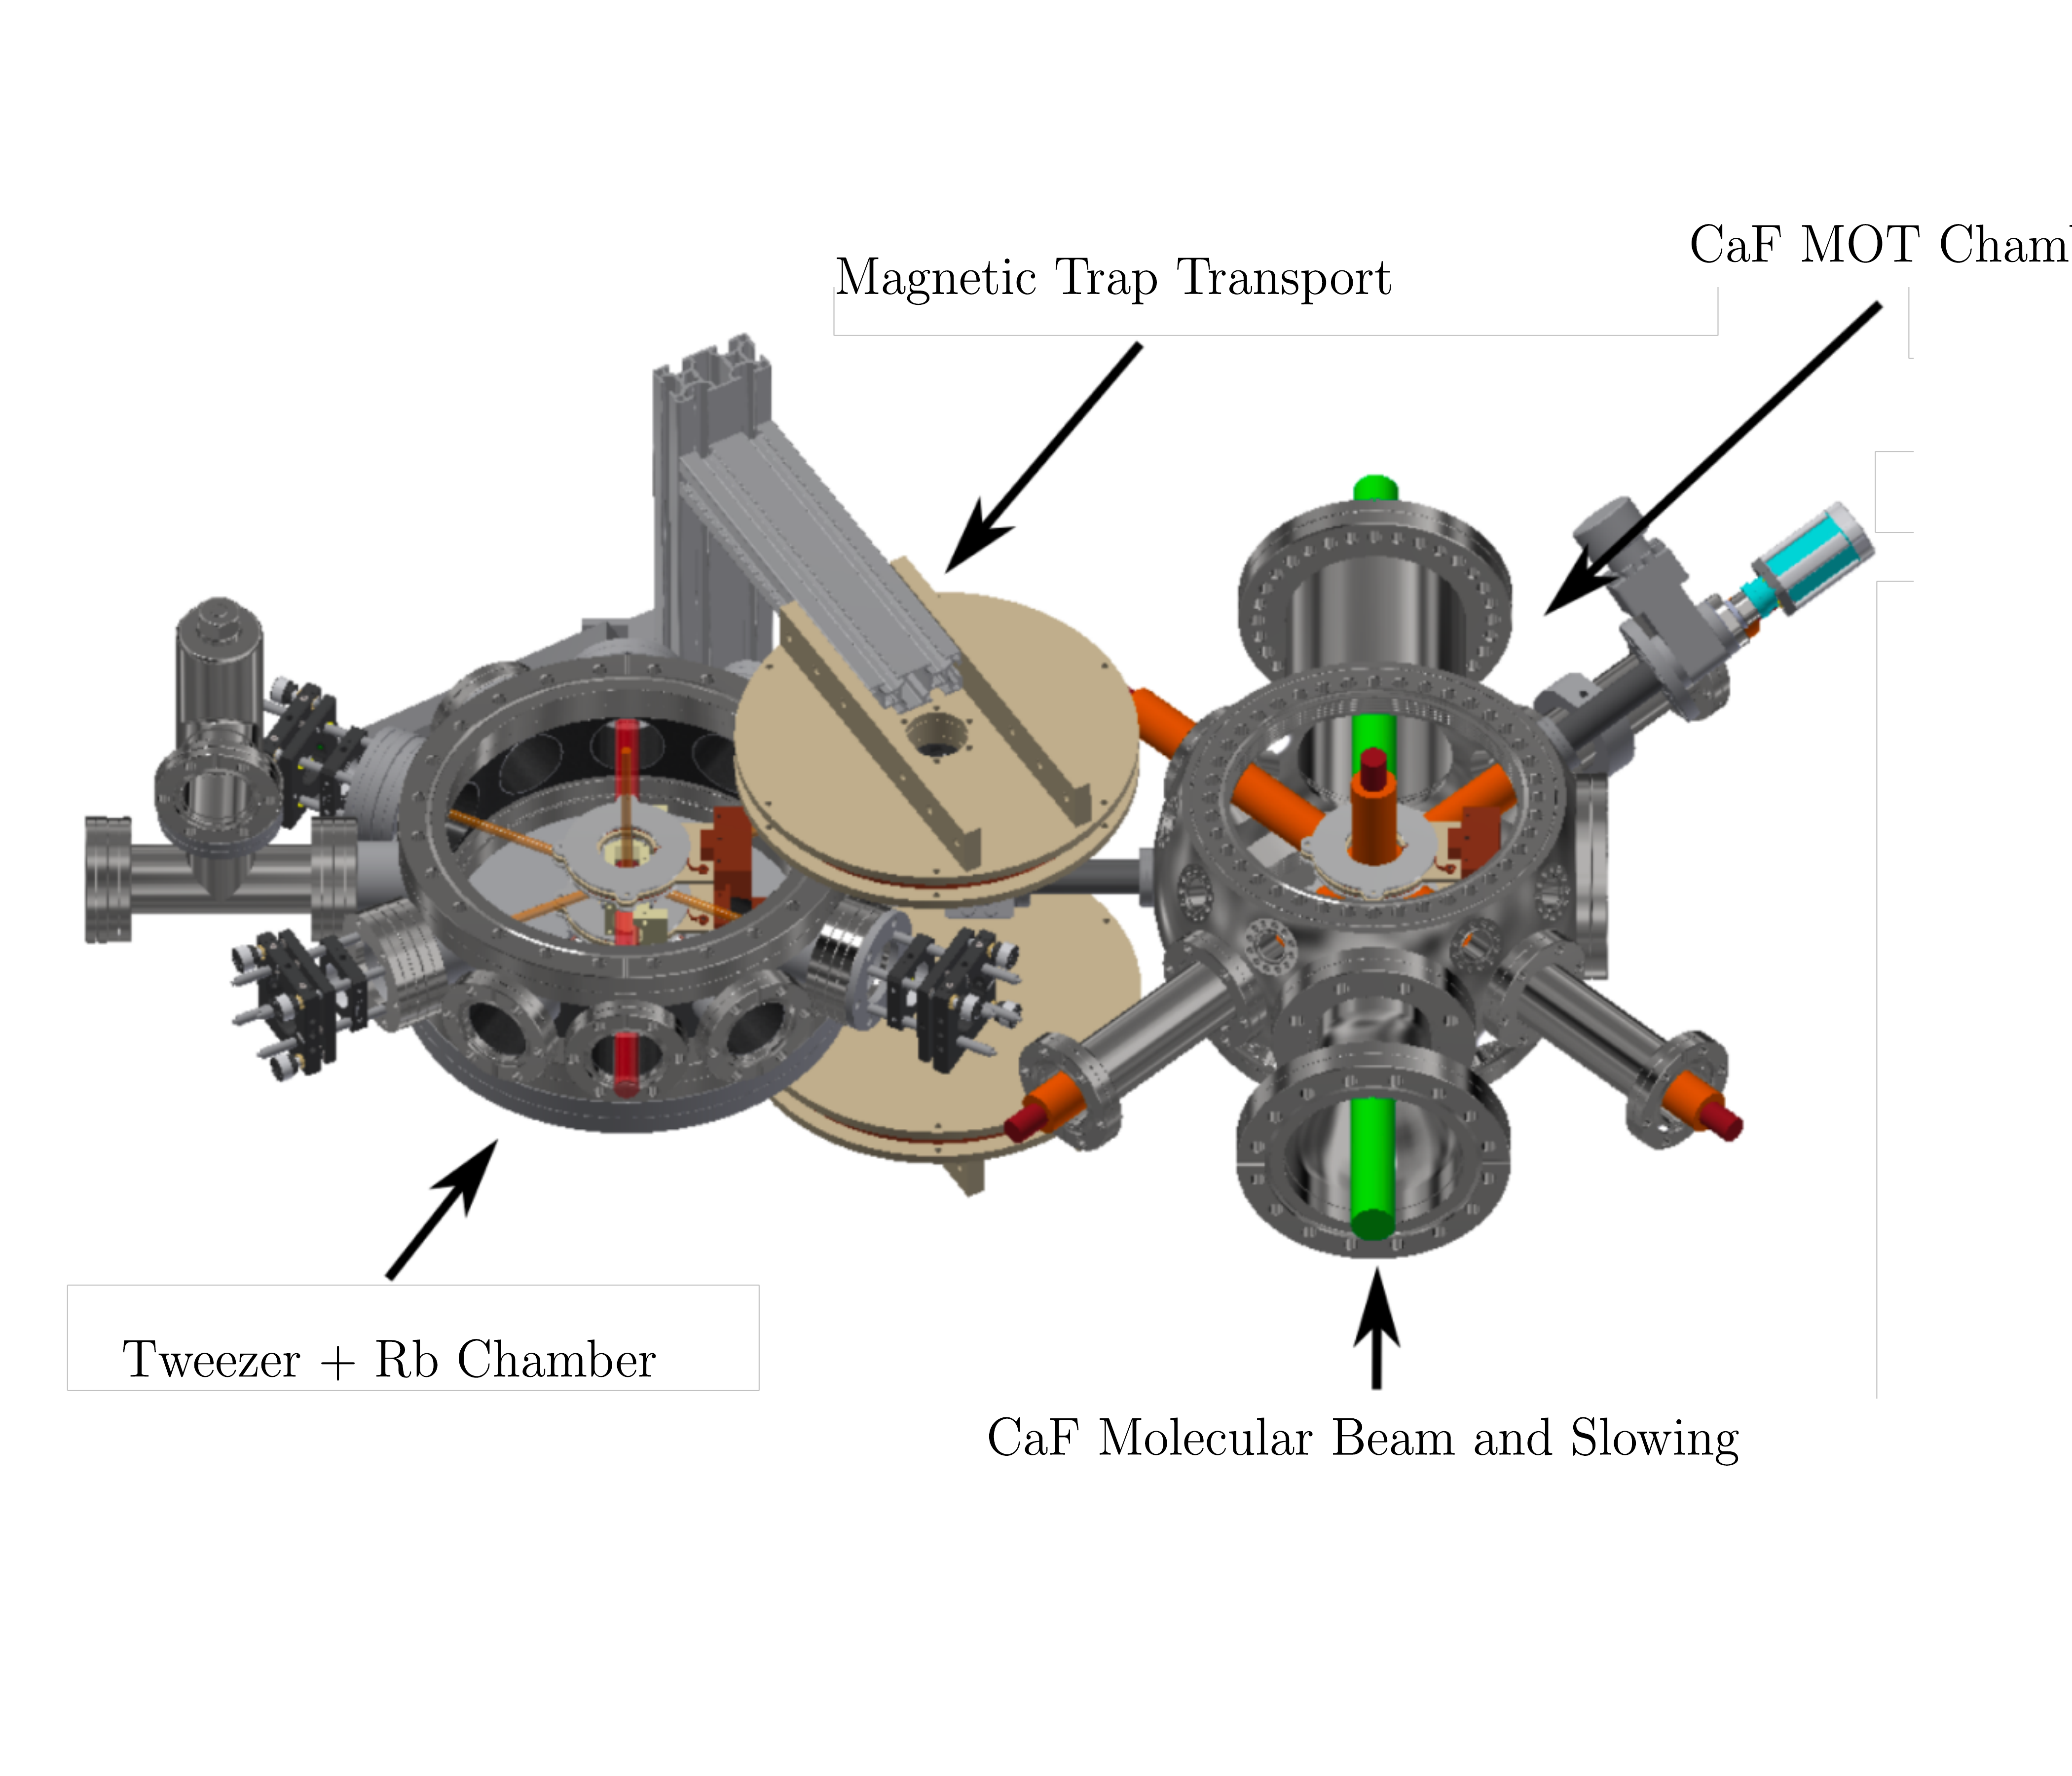
\includegraphics[width=\linewidth]{qsmol_figs/crop-31.png}
		\end{column}
	\end{columns}
\end{frame}

%------------------------------------------------

% \begin{frame}
% 	\frametitle{Trapping CaF Molecules}

% 
\includegraphics[width=\linewidth]{Images/blue_mot_slide.png}
% \end{frame}

%------------------------------------------------

\begin{frame}
	\frametitle{Second Wavelength Tweezer Array}

	\begin{columns}[T]
		\begin{column}{0.42\linewidth}
			\small
			\begin{itemize}
				\item Set up a second high-speed SLM for generating an array which is selectively attractive to CaF.
				\item Small site spacing of \textasciitilde 1.0 um between CaF and Rb without interference.
				\item Species selective trapping.
			\end{itemize}

			\vspace{6pt}
			\textbf{Electric Field Control}
			\begin{itemize}
				\item Replace internal mount - install Faraday shielding and electrodes.
				\item Tuning the Rb Rydberg energy separation to match the CaF rotational energy separation for a resonant dipole interaction.
			\end{itemize}
		\end{column}
		\begin{column}{0.56\linewidth}
			\centering
			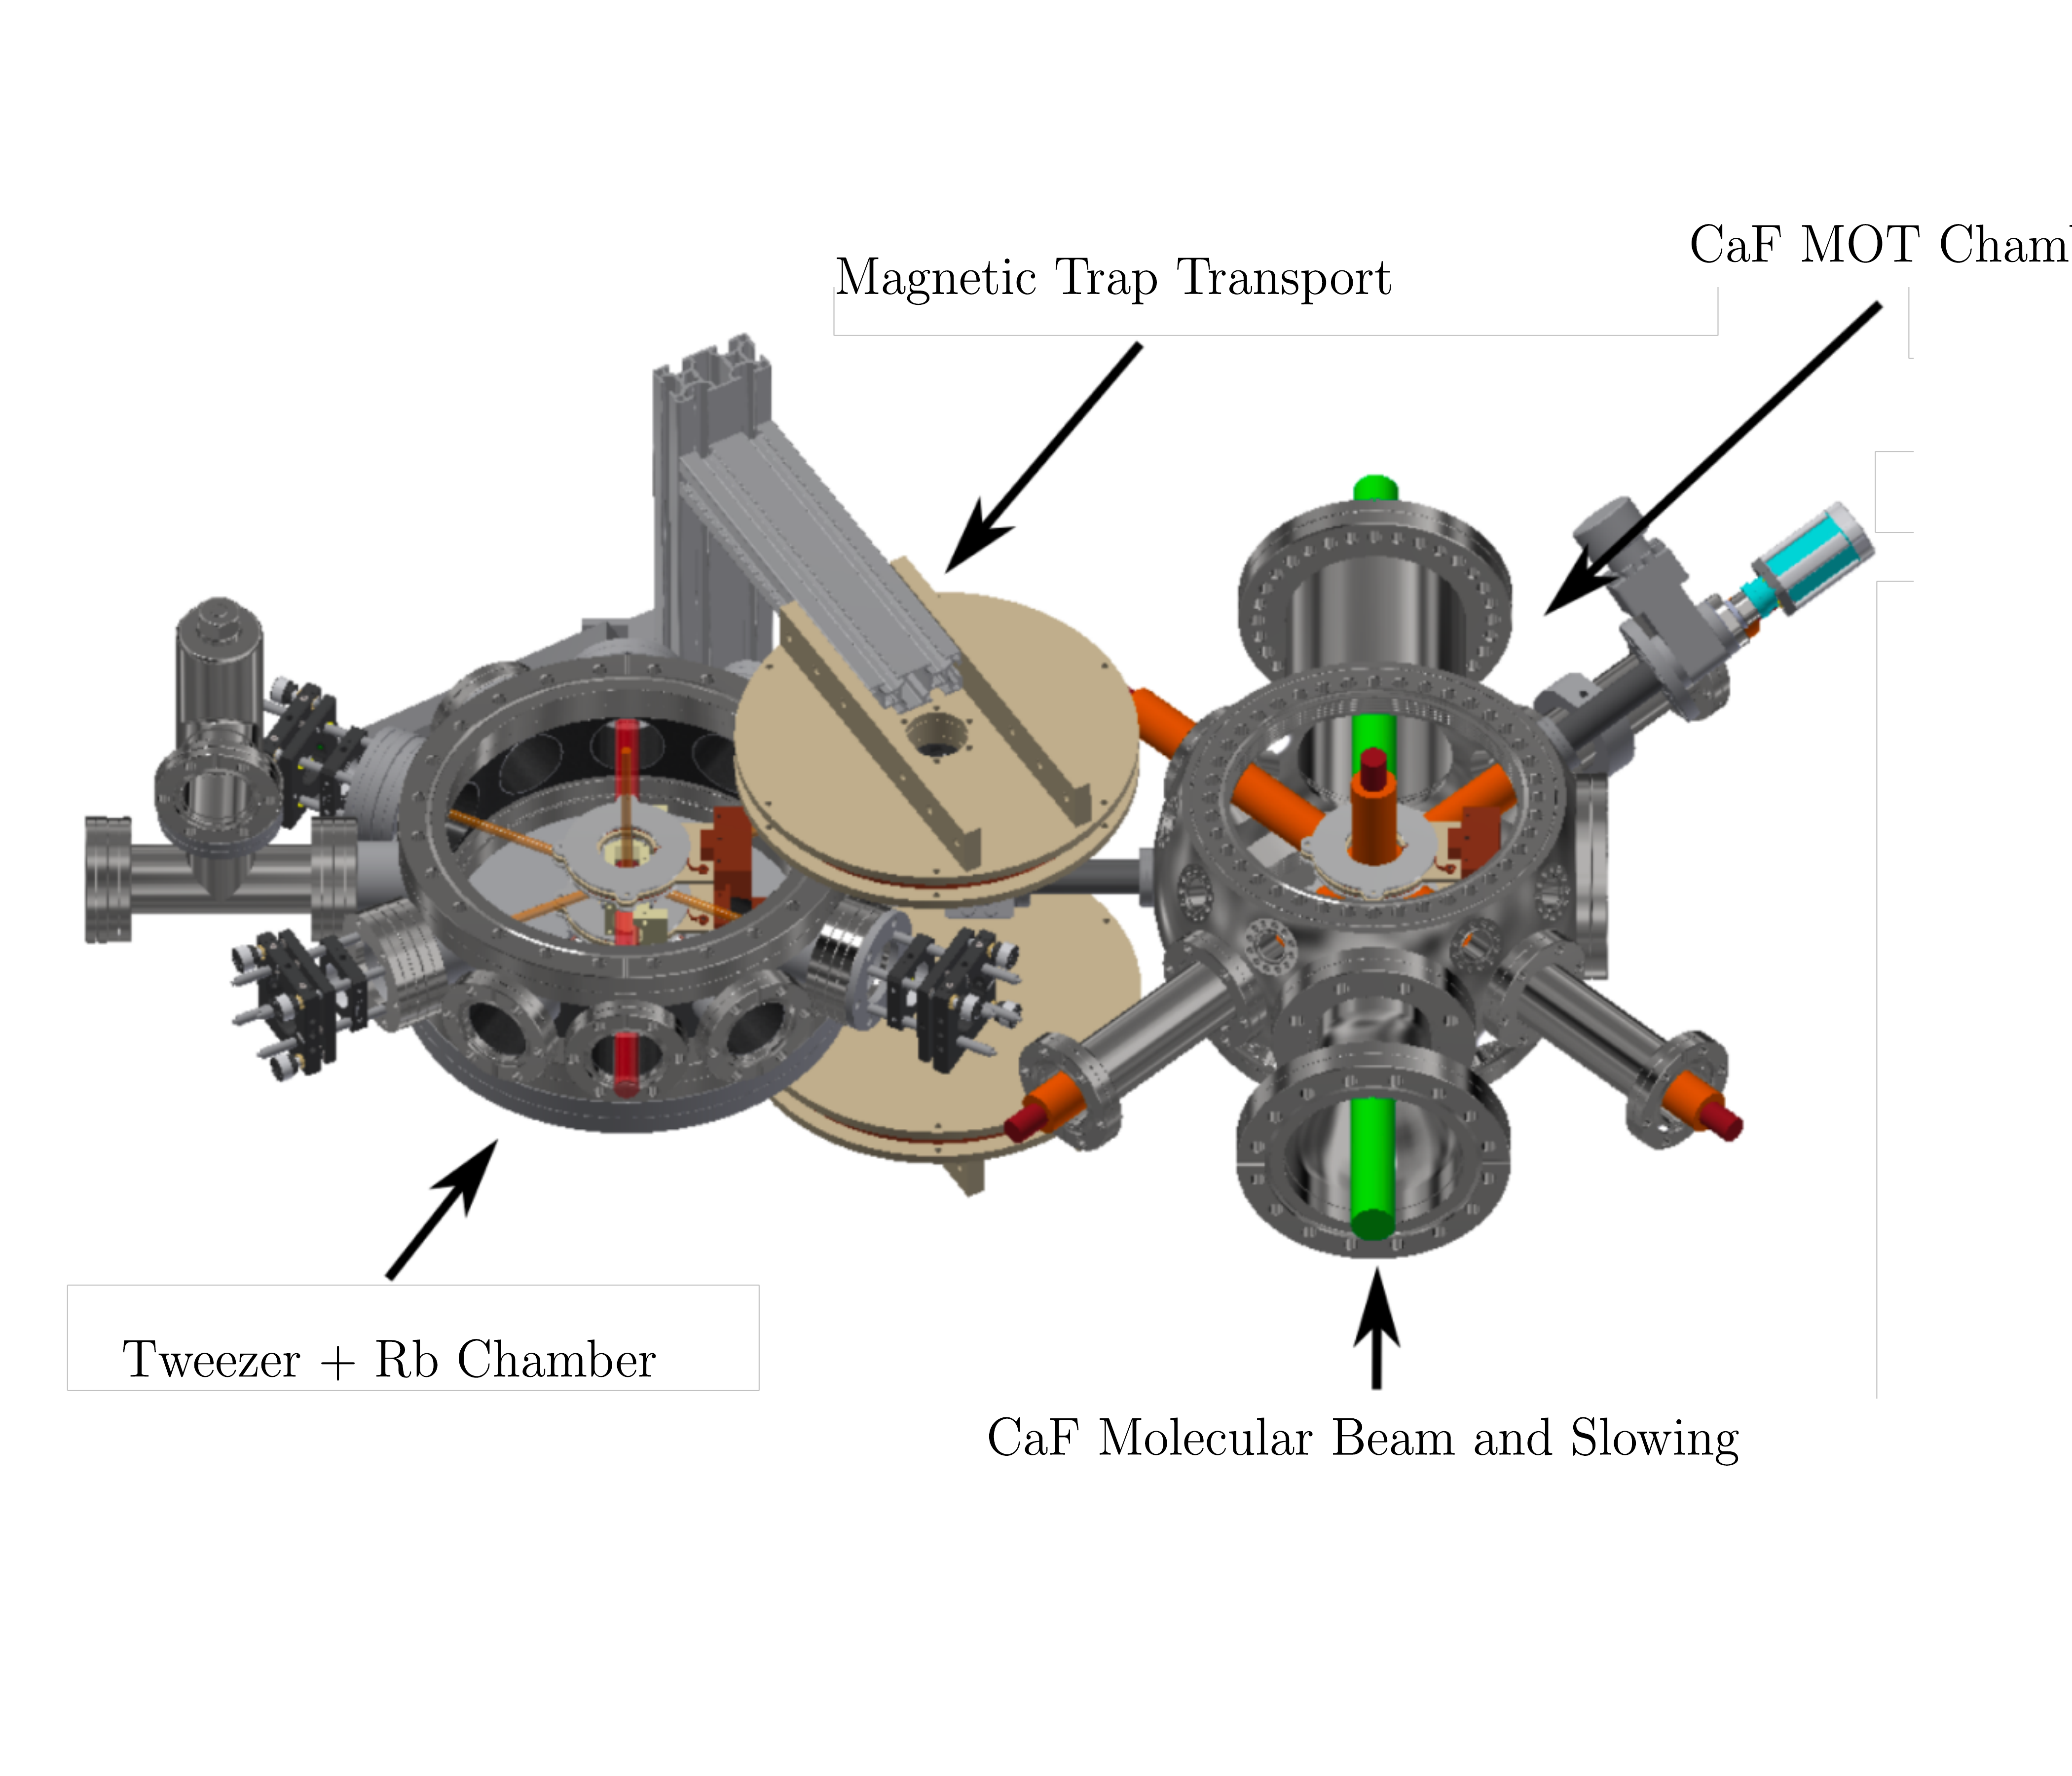
\includegraphics[width=\linewidth]{qsmol_figs/crop-31.png}
		\end{column}
	\end{columns}
\end{frame}


%----------------------------------------------------------------------------------------
%	HIGH-SPEED PARALLEL REARRANGEMENT
%	(reused from the QSMol talk)
%----------------------------------------------------------------------------------------

\begingroup
	\setbeamercolor{background canvas}{bg=ICLBlue}
	\setbeamercolor{normal text}{fg=white}\usebeamercolor[fg]{normal text}
	\setbeamercolor{page number in head/foot}{fg=white}

	\begin{frame}
		{\Huge\textcolor{white}{{\ImperialSansSemiBold High-Speed Parallel Rearrangement}}}
	\end{frame}
\endgroup

%------------------------------------------------

\begin{frame}
	\frametitle{Tweezer Array Rearrangement}

	\begin{columns}[T]
		\begin{column}{0.42\linewidth}
			\small
			\begin{itemize}
				\item Stochastic loading of Rb (\textasciitilde55\%) and CaF (\textasciitilde30\%).
				\item High-speed parallel rearrangement for \textbf{near-deterministic defect-free arrays} in arbitrary geometries.
				\item Pre-calculate initial and final array phase masks using full phase-retrieval algorithm (5 sec).
				\item Intermediate phase masks calculated by \textbf{linearly interpolating} trap weights, phases, positions.
				\item Map occupied trap sites to final trap sites using an \textbf{efficient sorting algorithm} (e.g. Hungarian, Jonker-Volgenant algorithms).
			\end{itemize}
		\end{column}
		\begin{column}{0.56\linewidth}
			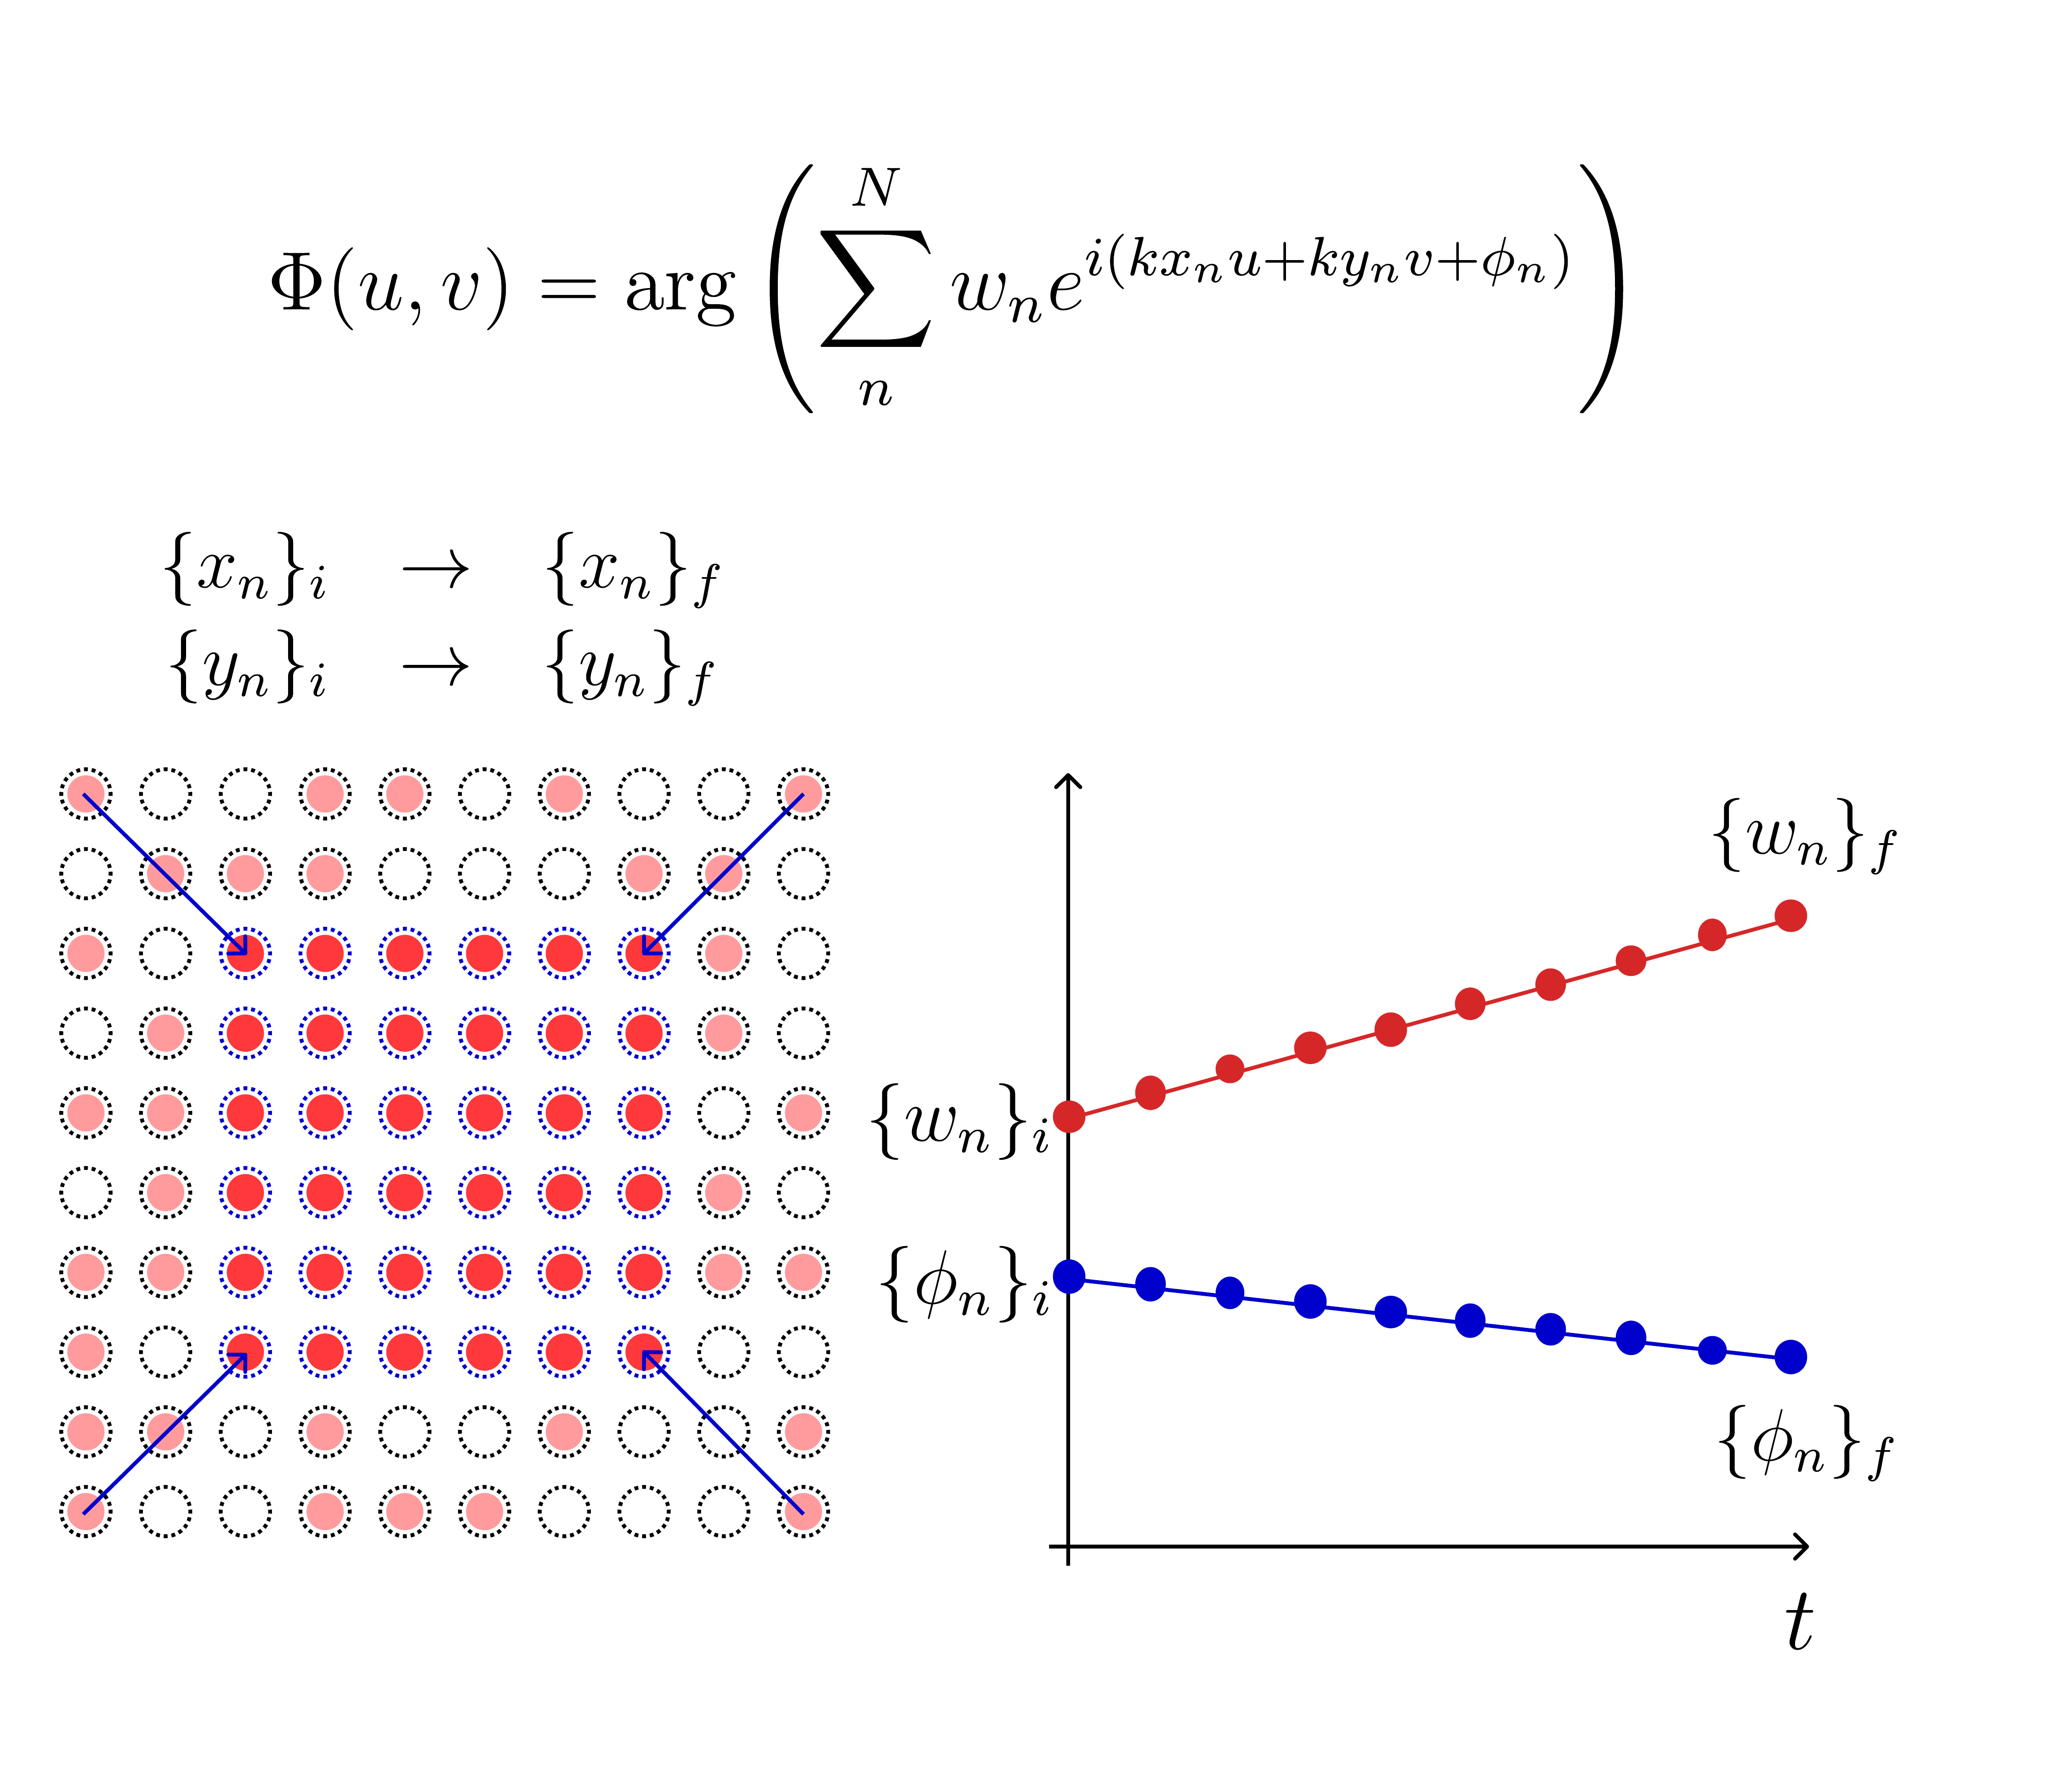
\includegraphics[width=0.9\linewidth]{qsmol_figs/crop-22.png} 

			\tiny Knottnerus, Ivo, et al. "Parallel assembly of neutral atom arrays with an SLM using linear phase interpolation." SciPost Physics 19.4 (2025): 118.
		\end{column}
	\end{columns}

\end{frame}

%------------------------------------------------

\begin{frame}
	\frametitle{Tweezer Array Rearrangement}

	\begin{columns}[T]
		\begin{column}{0.42\linewidth}
			\small
			\begin{enumerate}
				\item Load and image tweezer array (20 ms exposure).
				\item Process image and extract occupancy mask of array (2 ms).
				\item Map occupied trap sites to final trap sites using JV sorting algorithm (\textless1ms).
				\item Switch off unoccupied and excess trap sites.
				\item Interpolate, calculate next phase mask + upload phase mask to SLM (in parallel, \textasciitilde1.8 ms per frame, typ. 20 ms total rearrangement time).
			\end{enumerate}
		\end{column}
		\begin{column}{0.56\linewidth}
			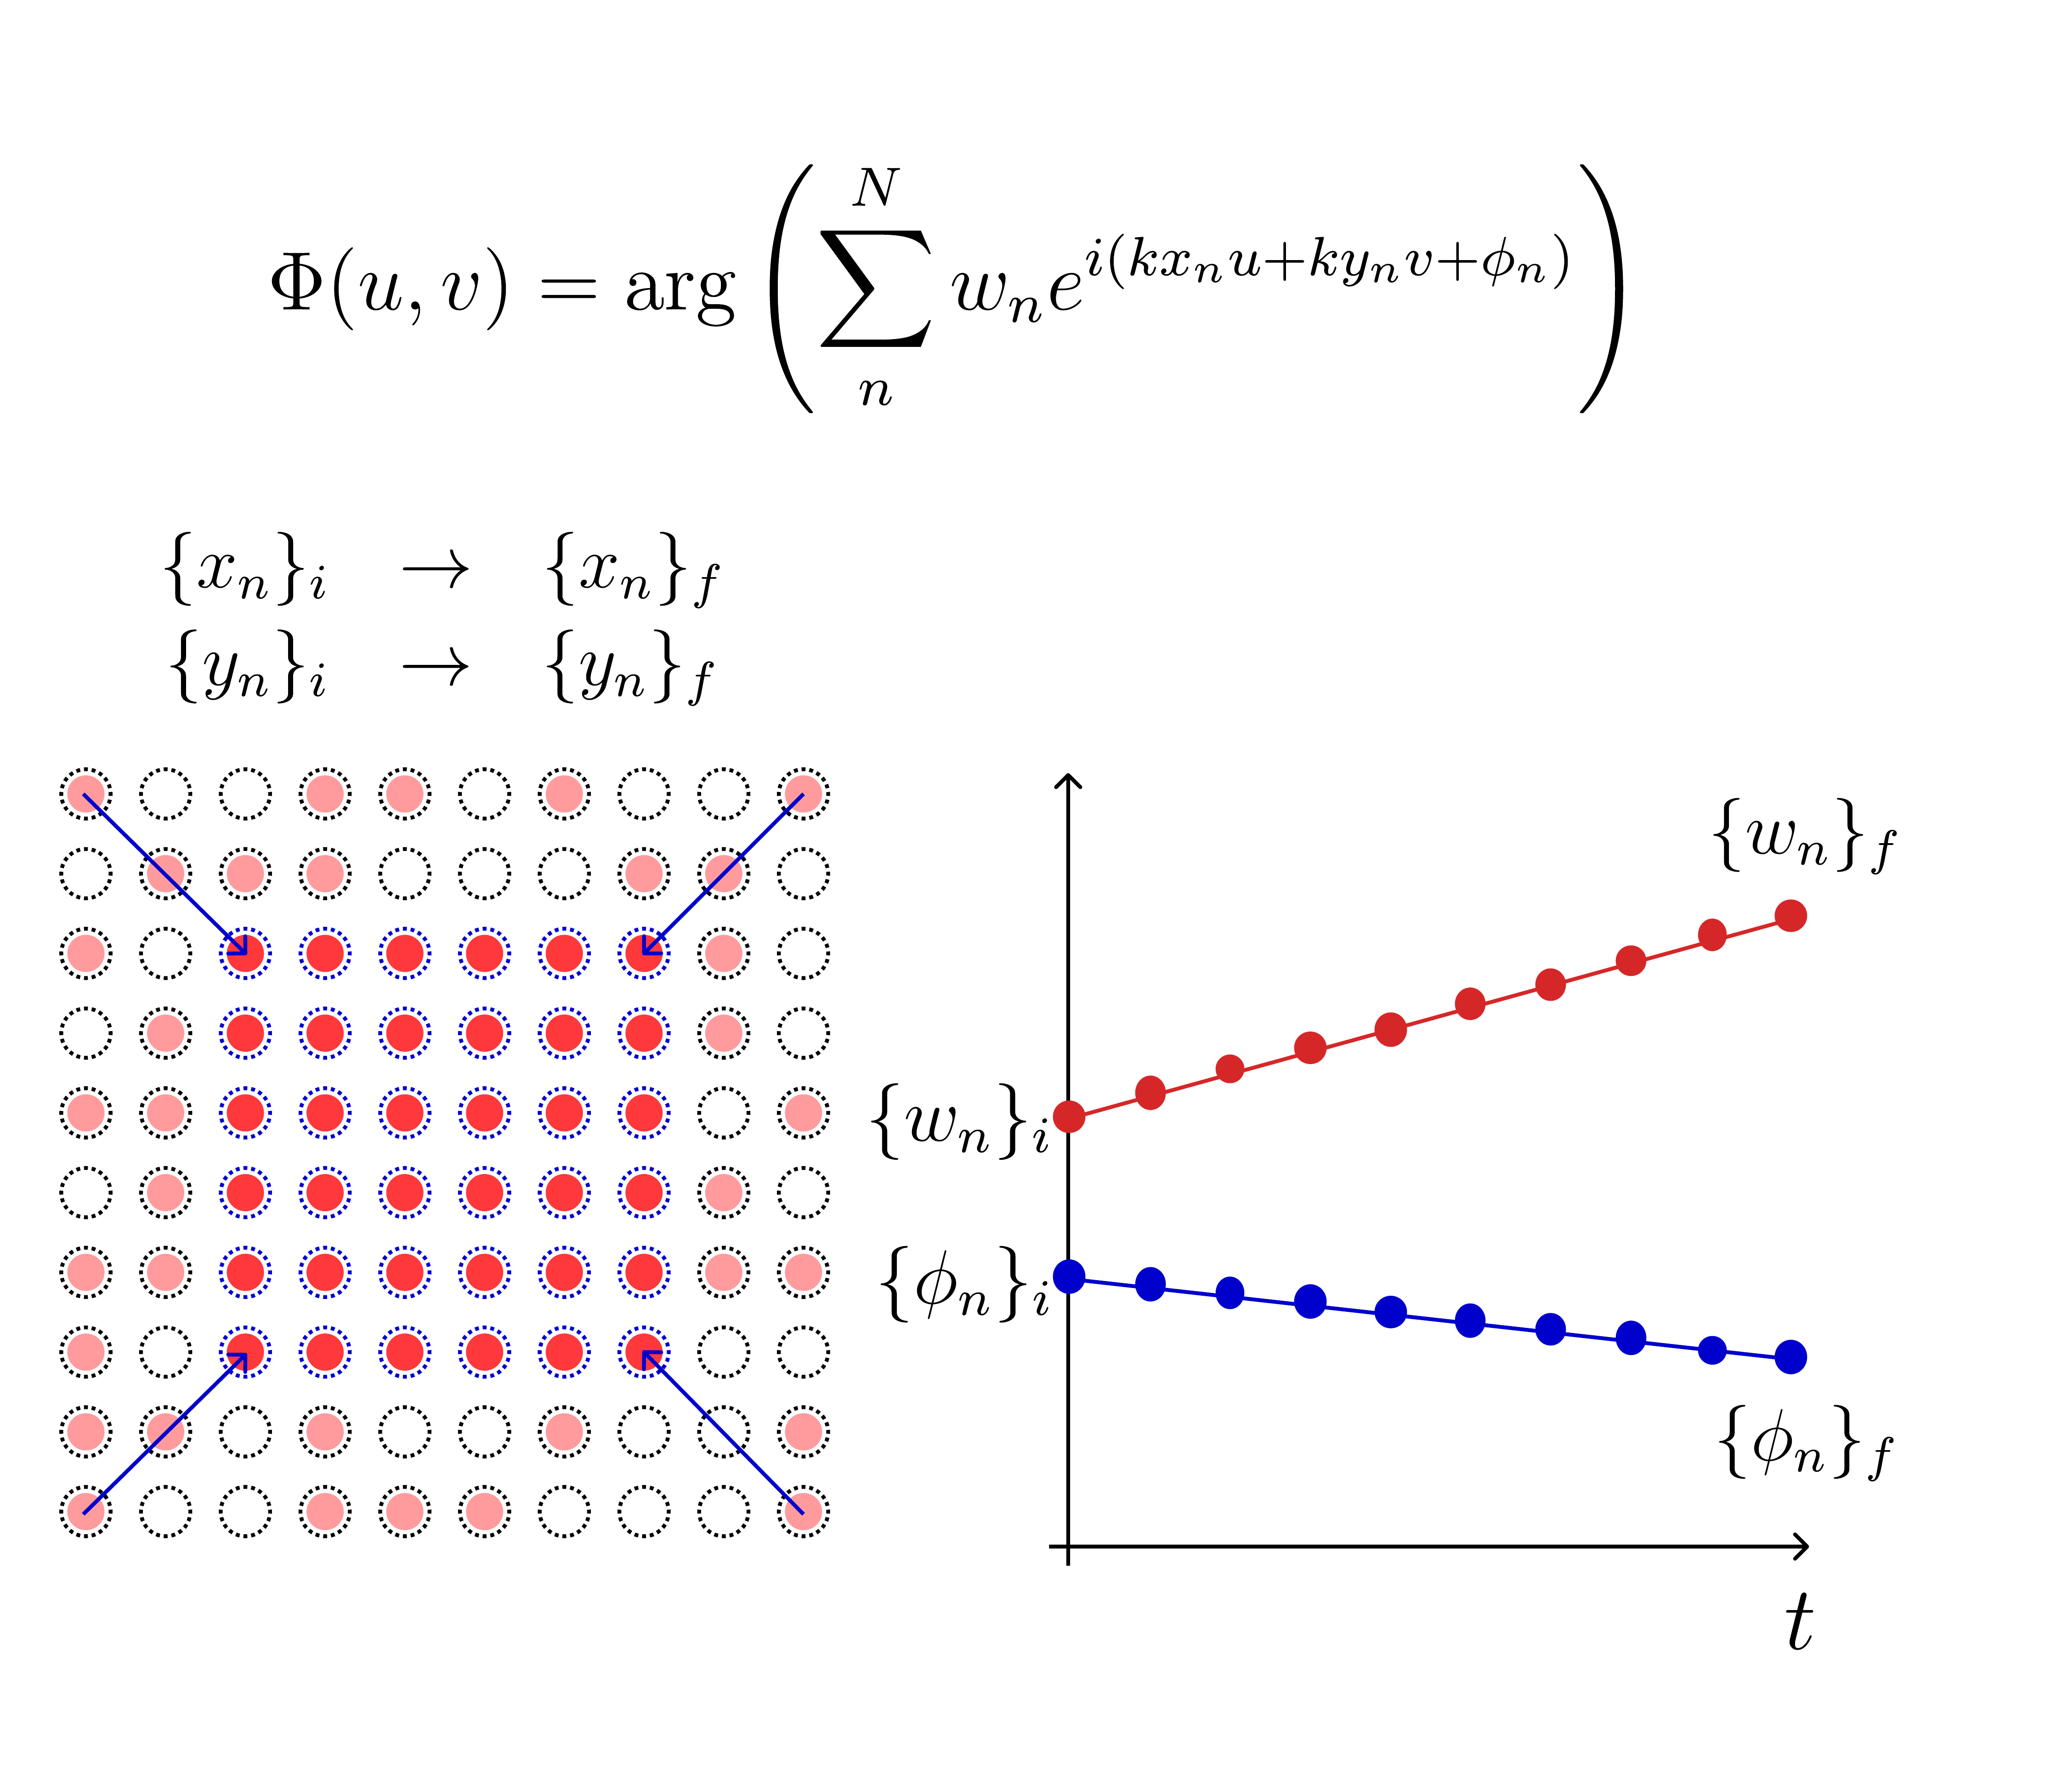
\includegraphics[width=\linewidth]{qsmol_figs/crop-22.png}
		\end{column}
	\end{columns}
\end{frame}

%------------------------------------------------

\begin{frame}
	\frametitle{Tweezer Array Rearrangement}
	\framesubtitle{Rearrangement Performance}

	\begin{columns}[T]
		\begin{column}{0.68\linewidth}
			\centering
			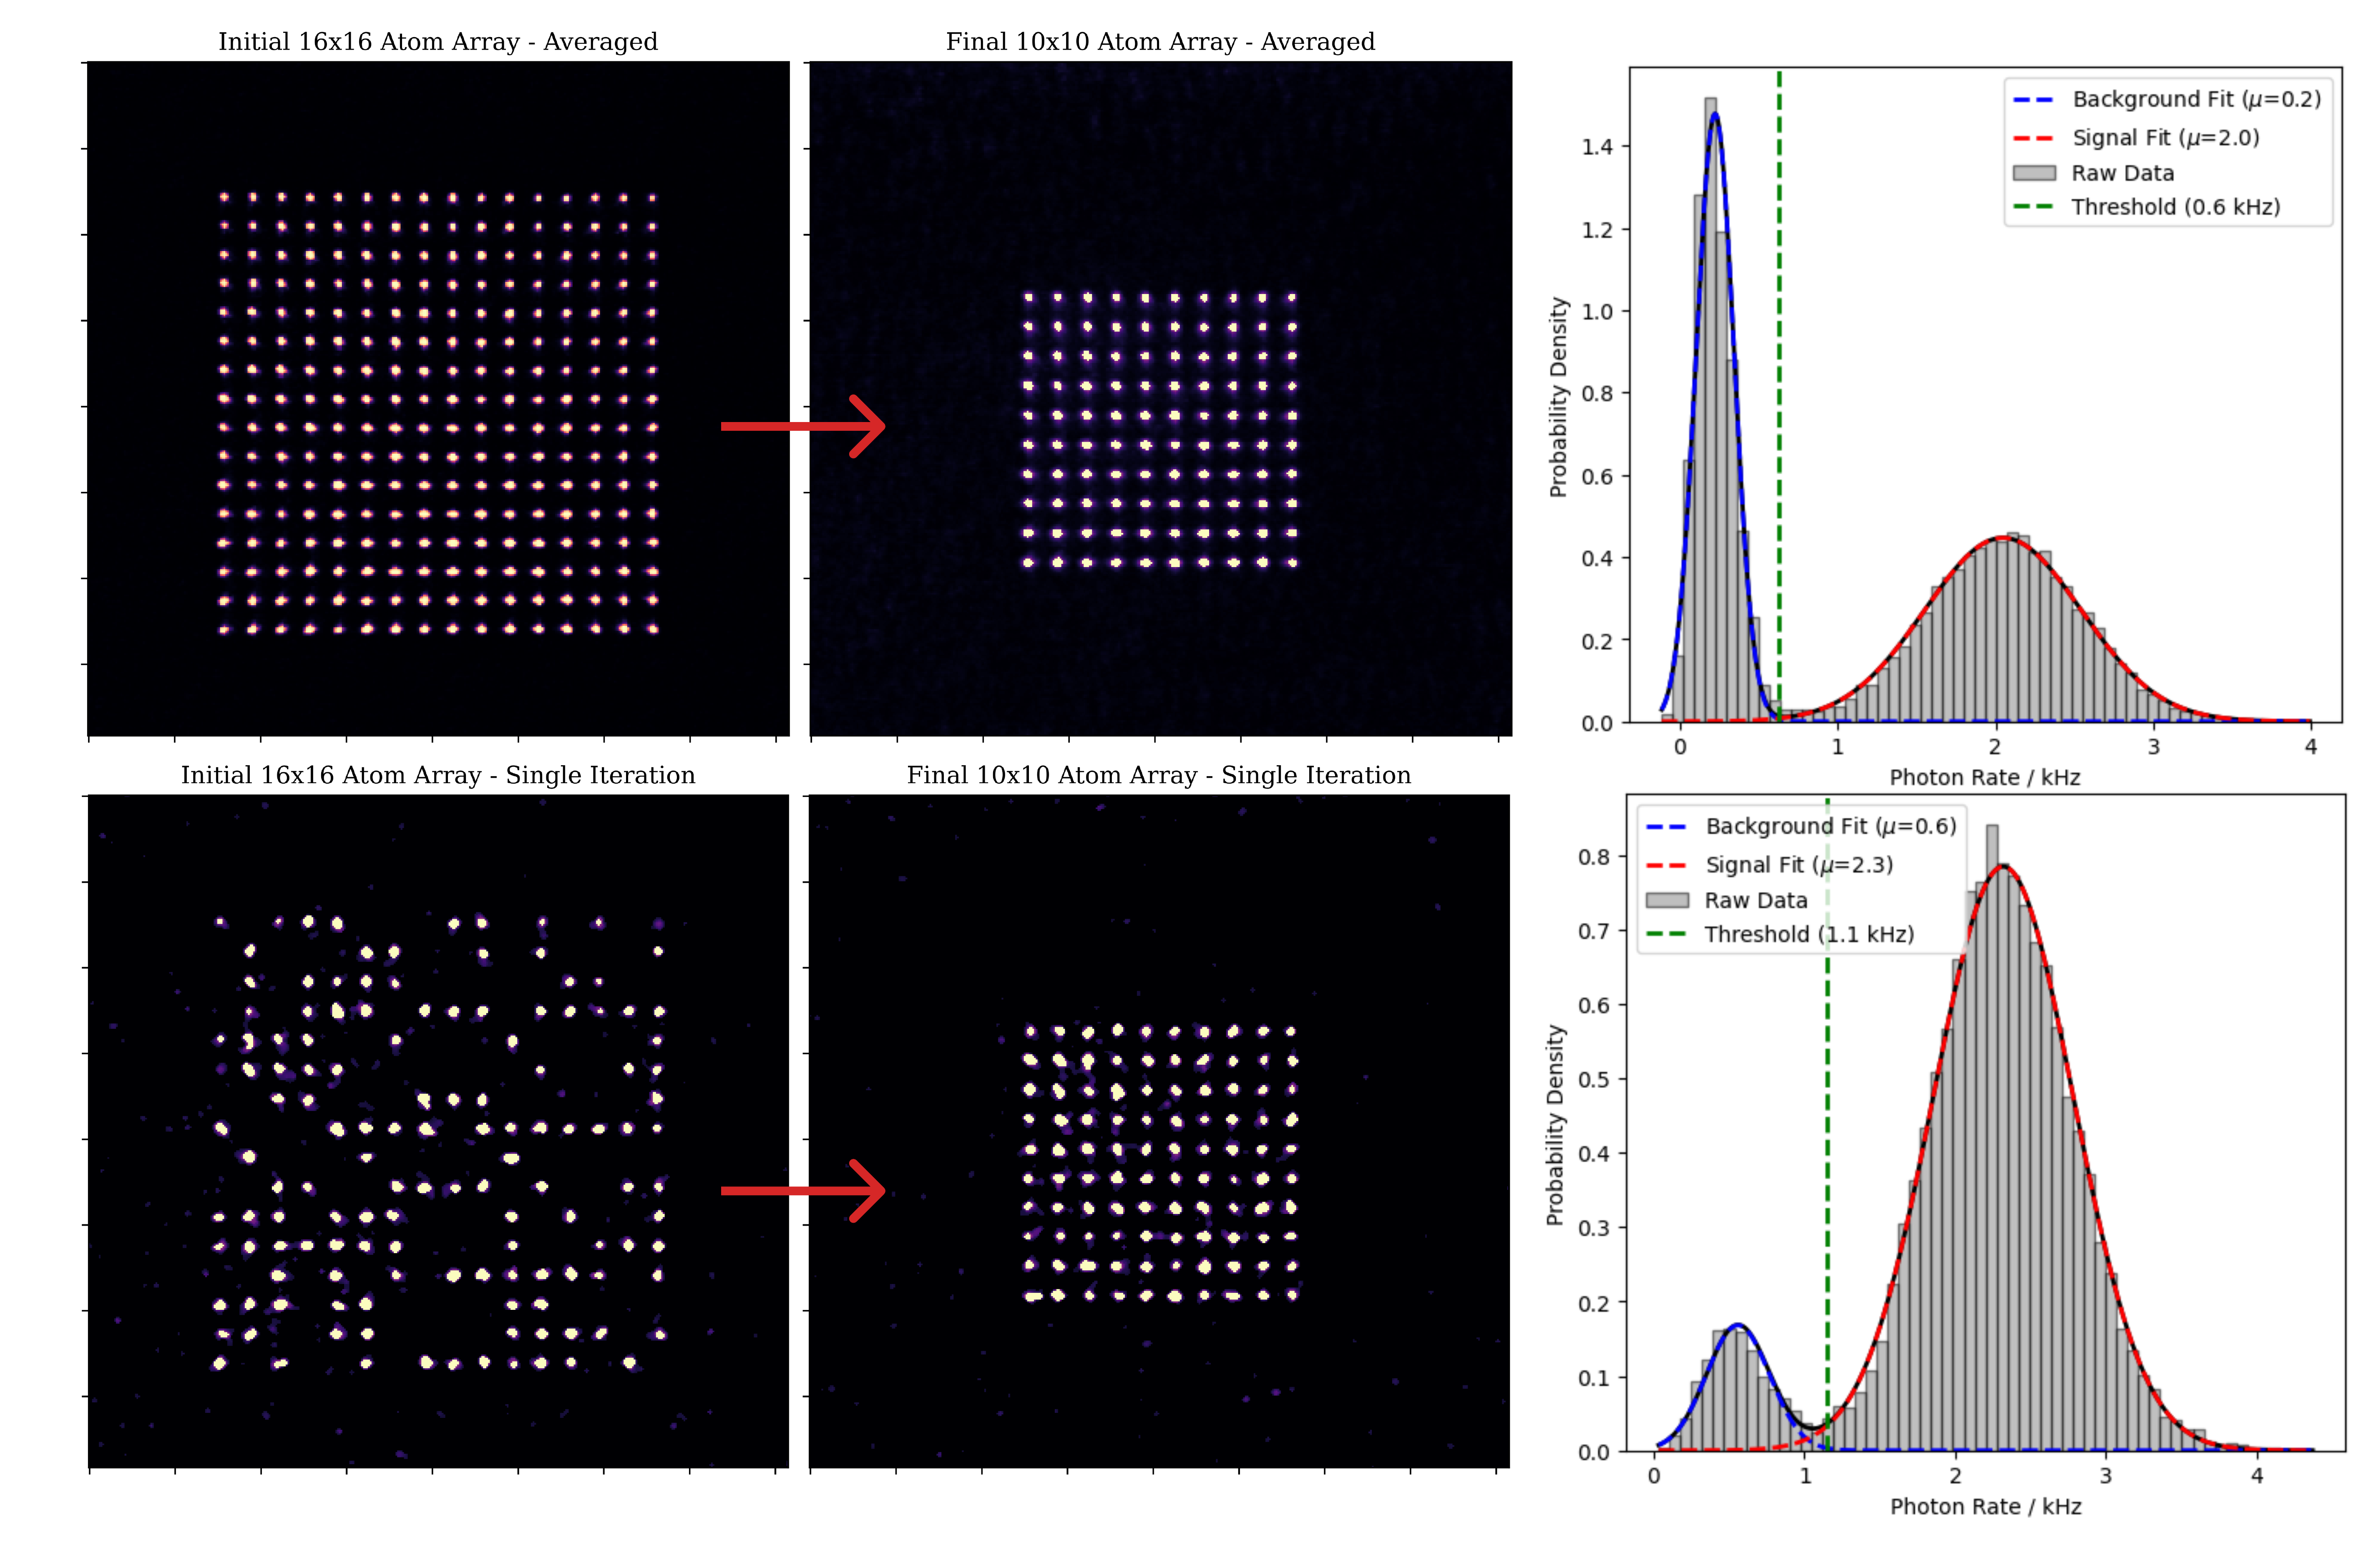
\includegraphics[width=\linewidth]{qsmol_figs/crop-25-notext.png}
		\end{column}
		\begin{column}{0.3\linewidth}
			\small
			\vspace{20pt}
			Initial array - 16x16 5.0um spacing\\
			\textbf{Mean filling fraction \textasciitilde 55\%}

			\vspace{50pt}
			Final array - 10x10 5.0um spacing\\
			\textbf{Mean filling fraction \textasciitilde 94\%}
		\end{column}
	\end{columns}
\end{frame}

%------------------------------------------------

\begin{frame}
	\frametitle{Tweezer Array Rearrangement}
	\framesubtitle{Filling Fraction vs Step Size}

	\begin{columns}[T]
		\begin{column}{0.48\linewidth}
			\centering
			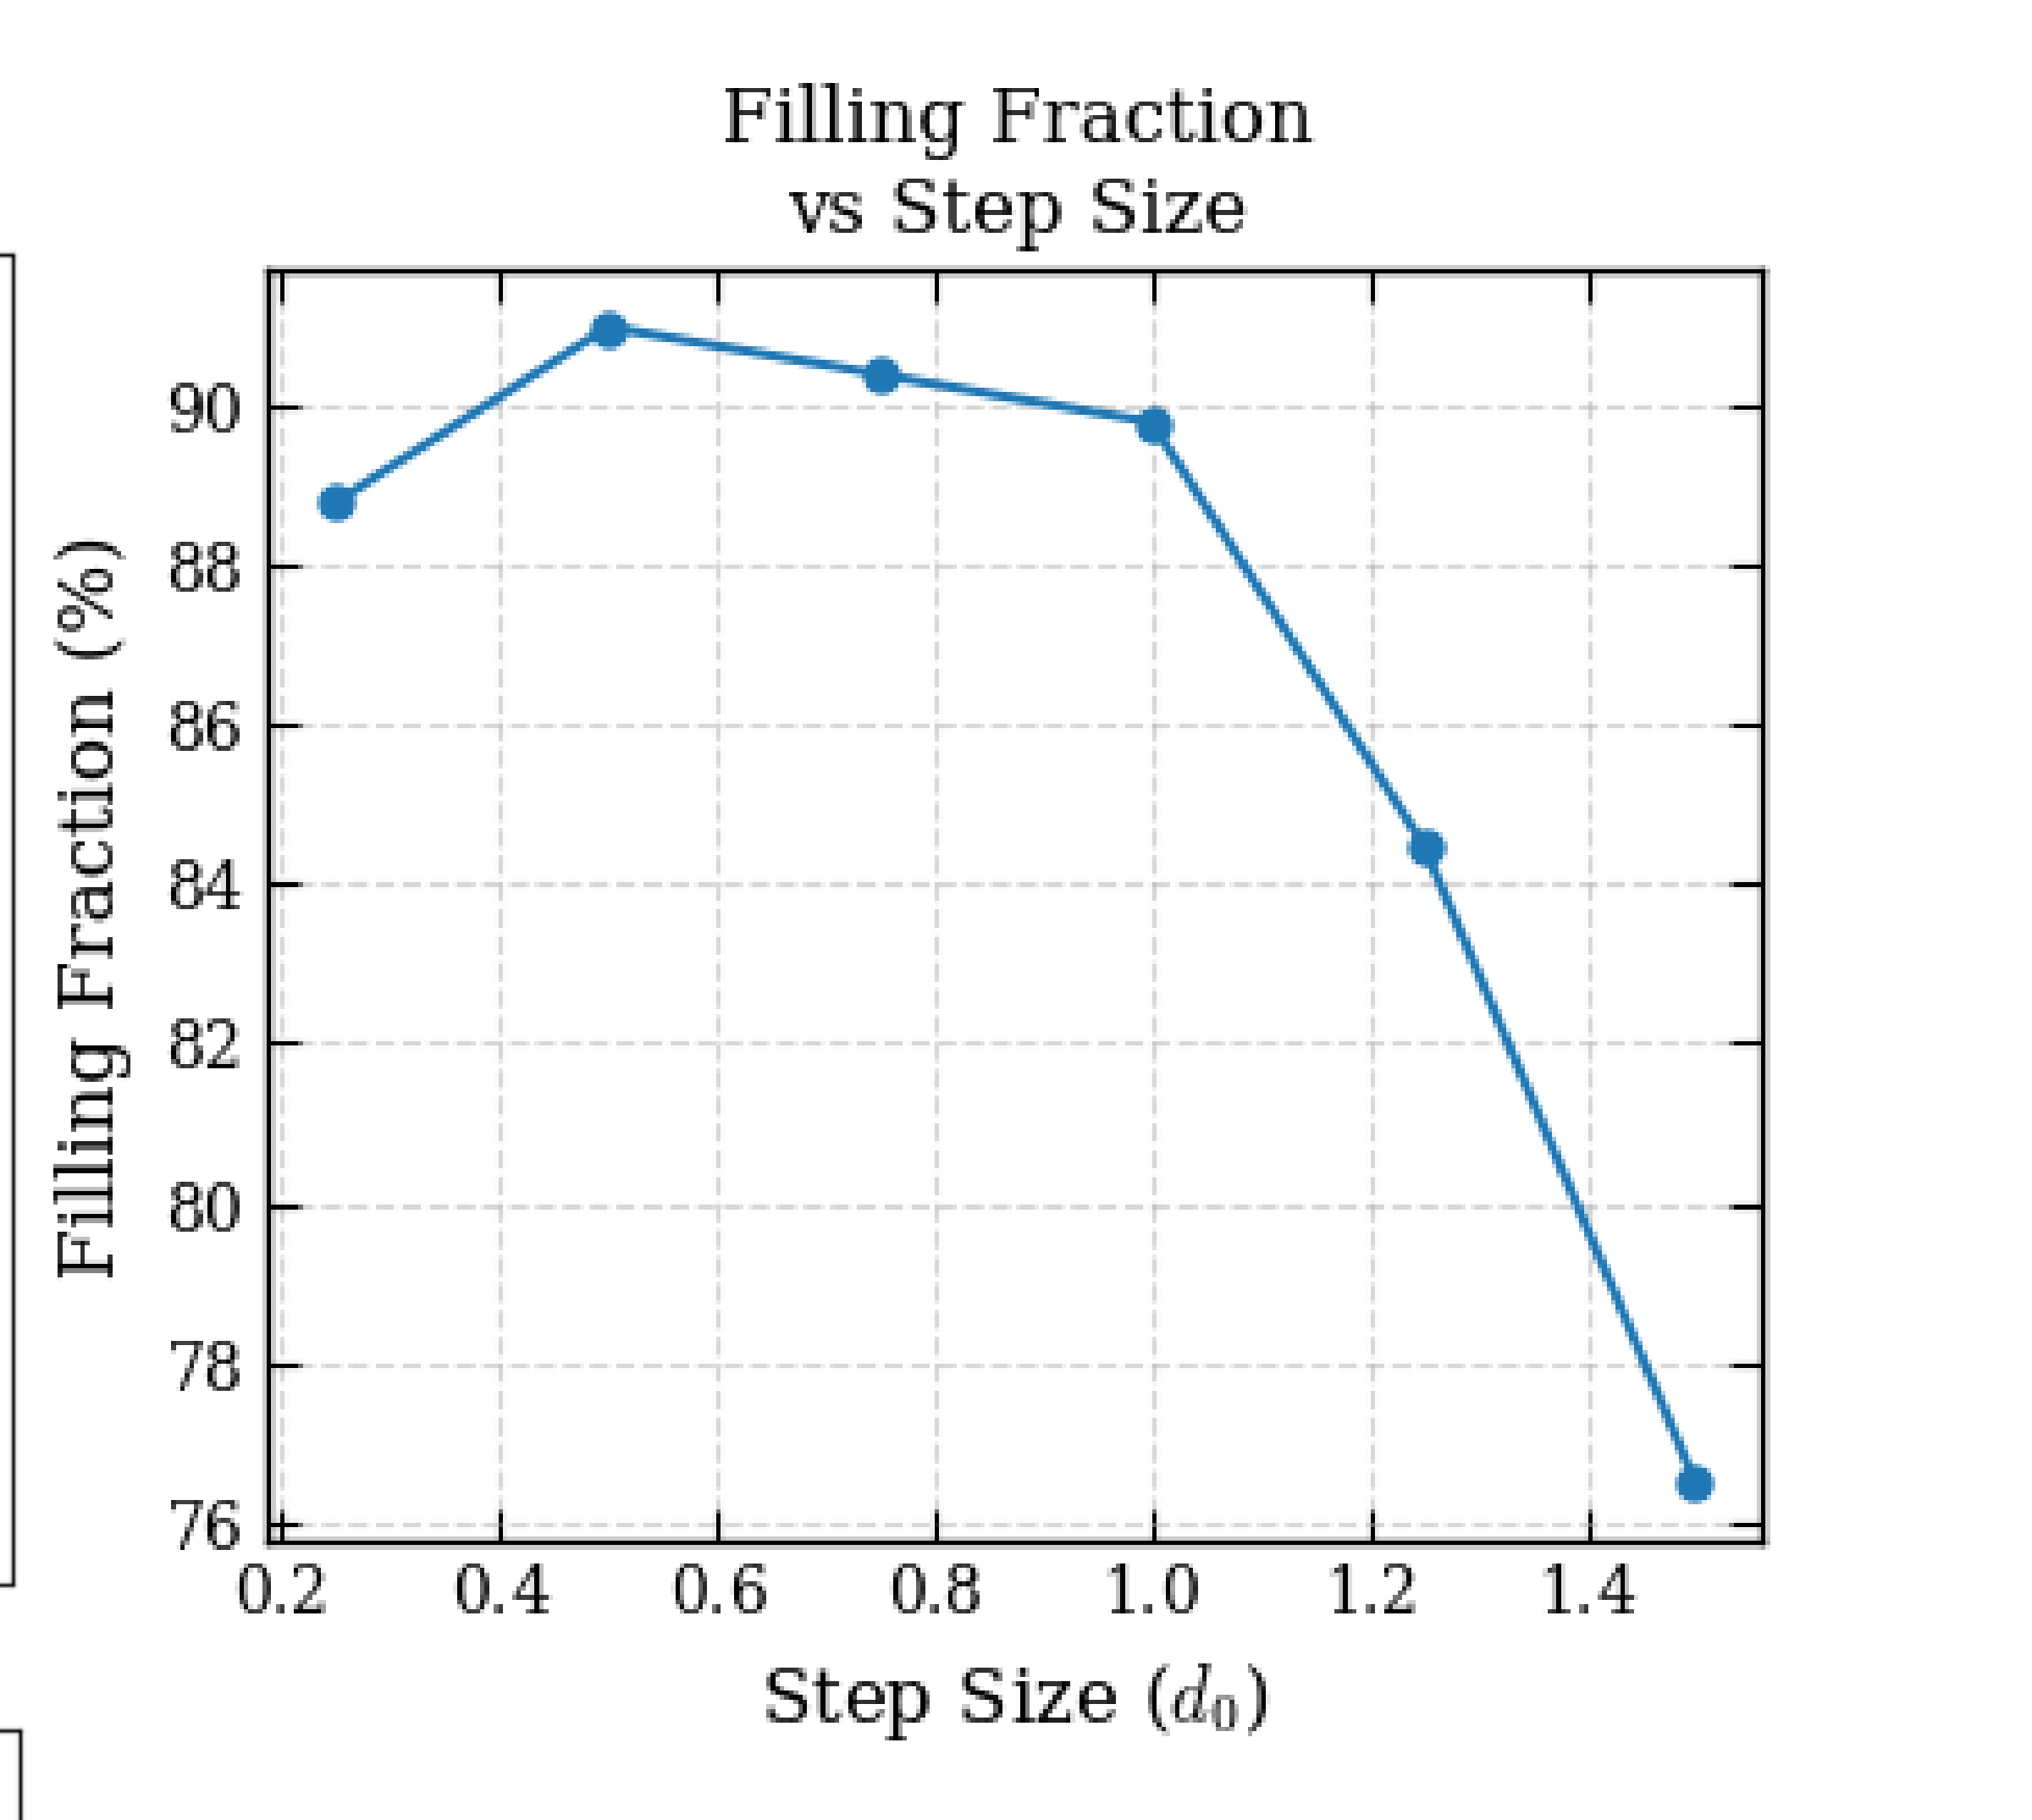
\includegraphics[width=\linewidth]{qsmol_figs/crop-26-fillfrac.png}
		\end{column}
		\begin{column}{0.48\linewidth}
			\small
			\begin{itemize}
				\item Max. step size \textasciitilde 1.0 um
				\item Rearrangement `speed' = 1.88 ms per frame
				\item 12.2 frames per sequence, 22.9 ms total rearrangement time
				\item Loss dominated by lifetime + imaging loss.
				\item Rearrangement `efficiency' \textasciitilde 98\%.
			\end{itemize}
		\end{column}
	\end{columns}
\end{frame}

%------------------------------------------------

\begin{frame}
	\frametitle{Dense Arrays}

	\begin{columns}[T]
		\begin{column}{0.42\linewidth}
			\small
			\textbf{For two-qubit hybrid gates need small trap site separation \textasciitilde 2.0 um for high-fidelity operations.}

			Challenges:
			\begin{itemize}
				\item Interference of tweezer light, deep off-plane traps, reduces detection fidelity.
				\item Interference between neighbouring trap sites, distorts trap potential.
				\item Rearrangement linear interpolation method breaks down for small site spacing.
			\end{itemize}
		\end{column}
		\begin{column}{0.56\linewidth}
			\centering
			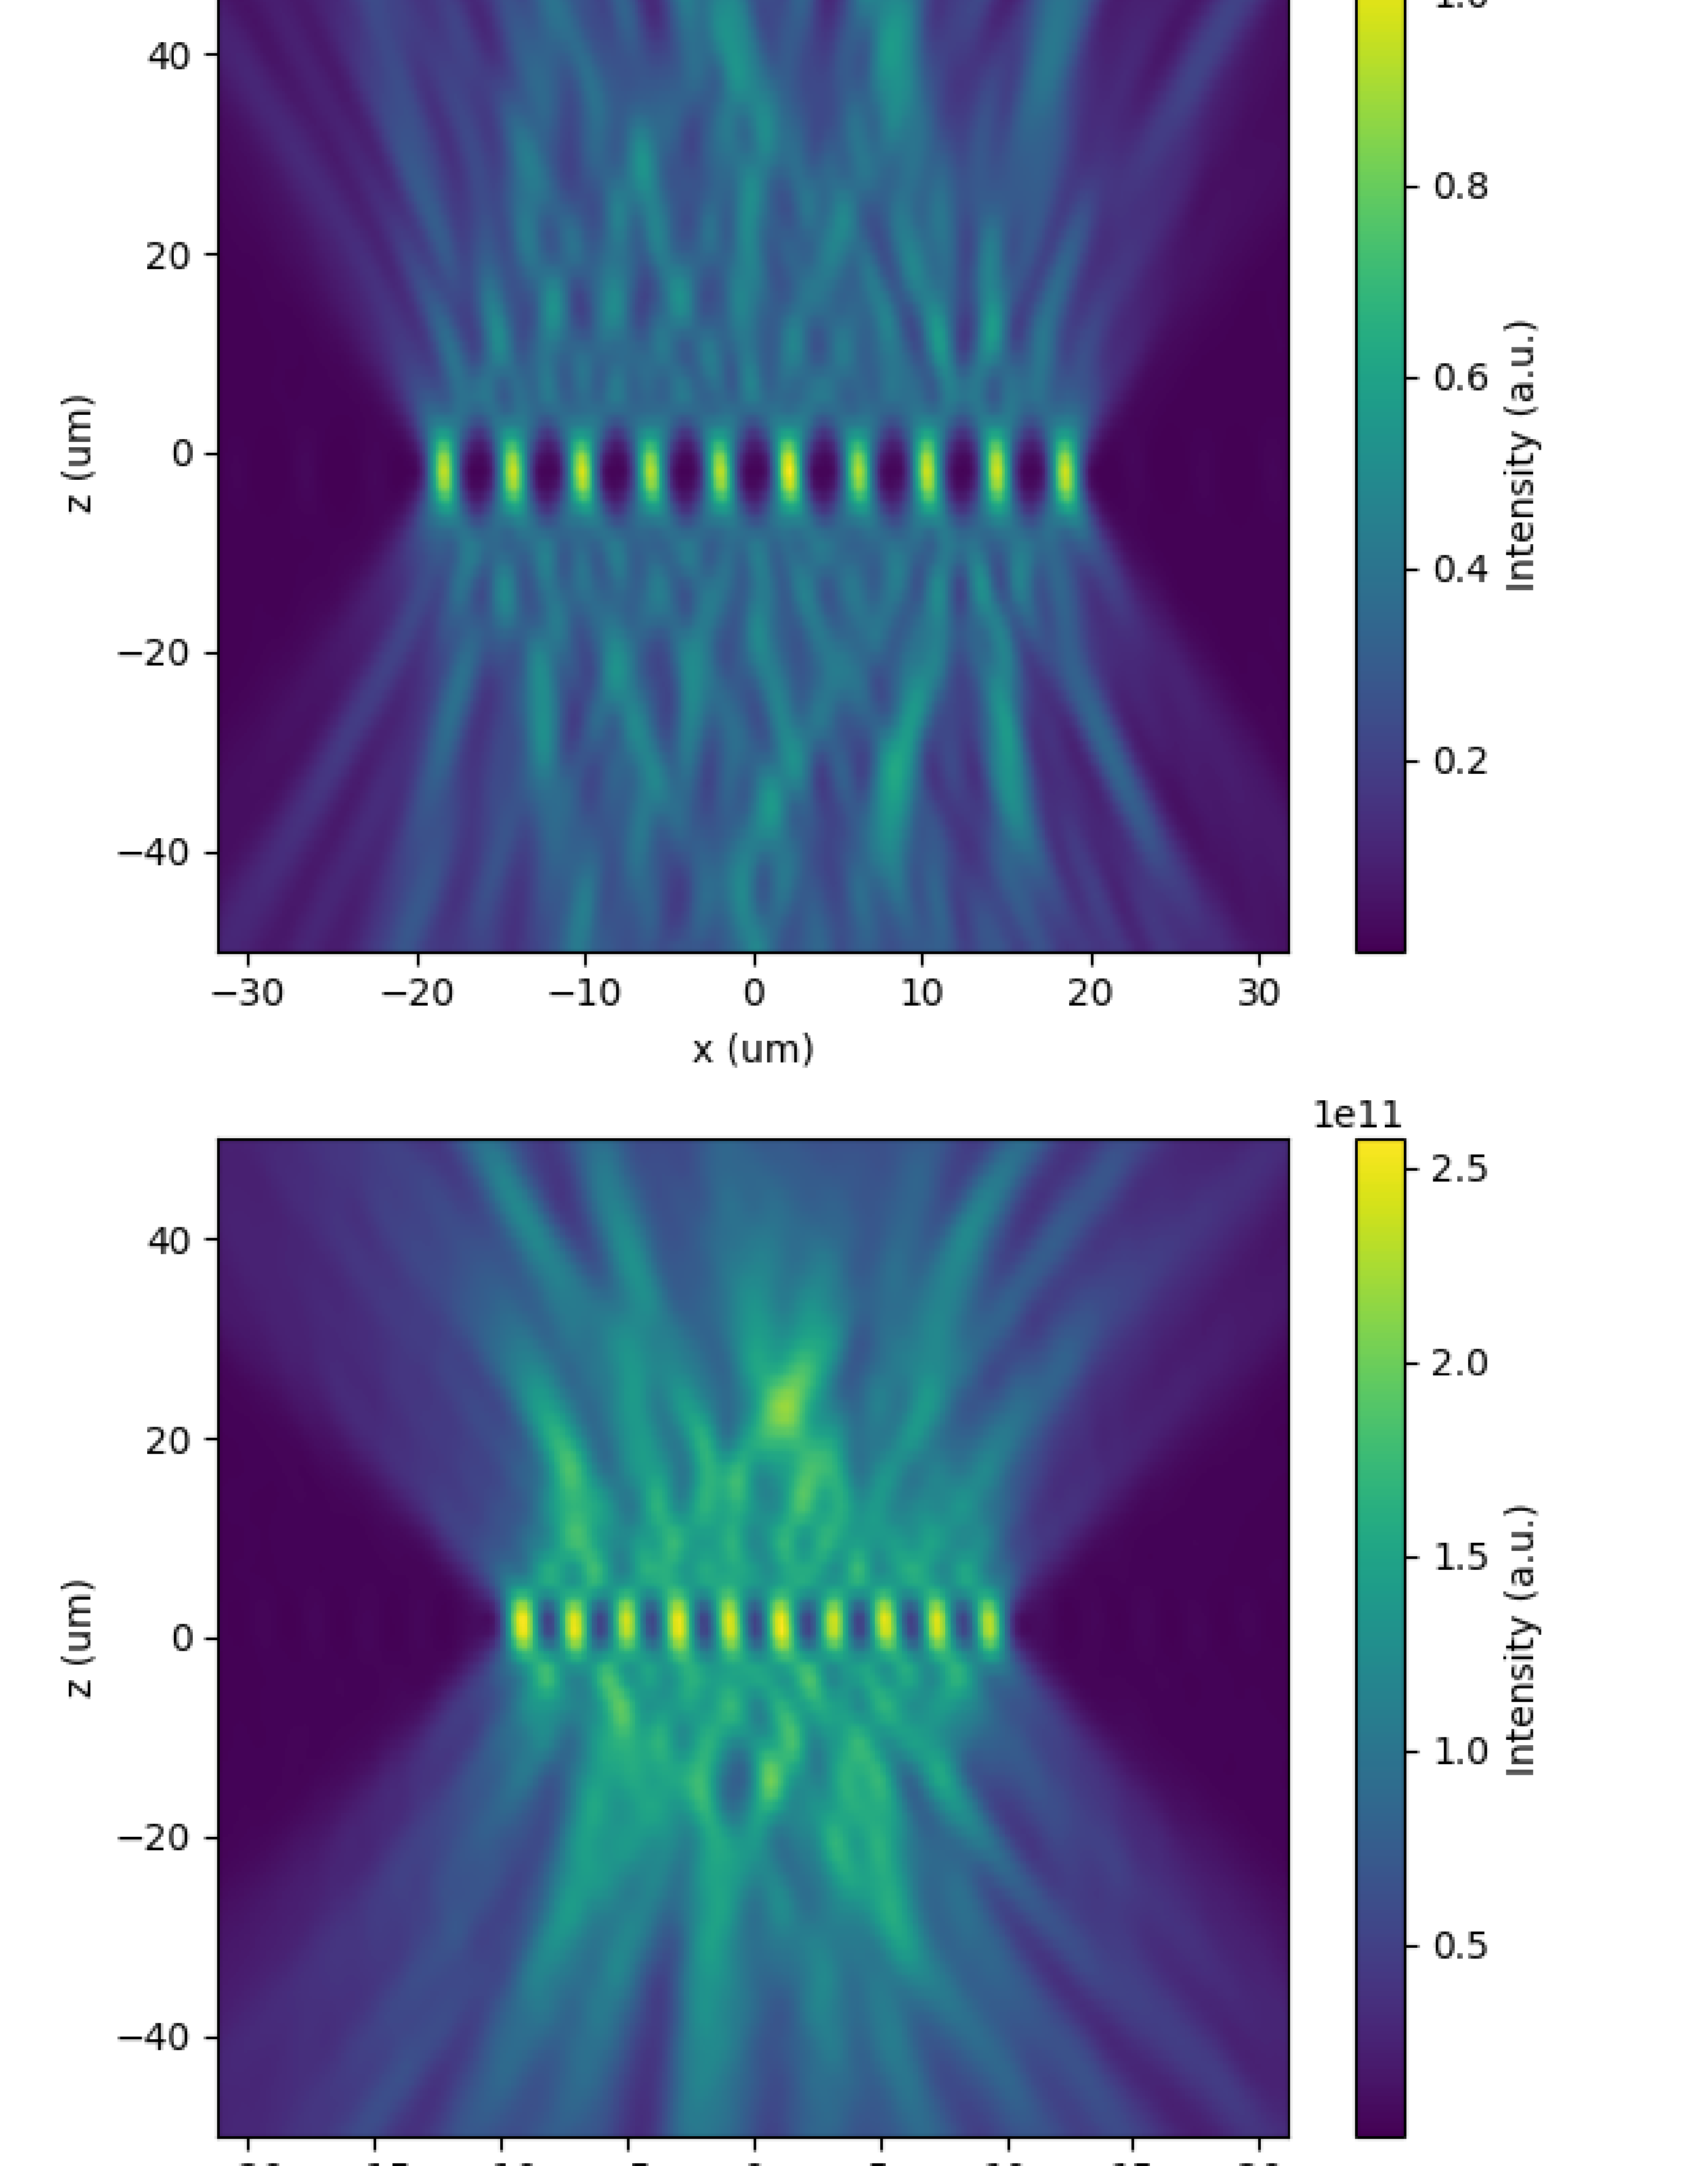
\includegraphics[width=0.85\linewidth, height=0.8\textheight, keepaspectratio]{qsmol_figs/crop-27-notext.png}
		\end{column}
	\end{columns}
\end{frame}



%------------------------------------------------

\begin{frame}
	\frametitle{Dense Arrays}

	\centering
	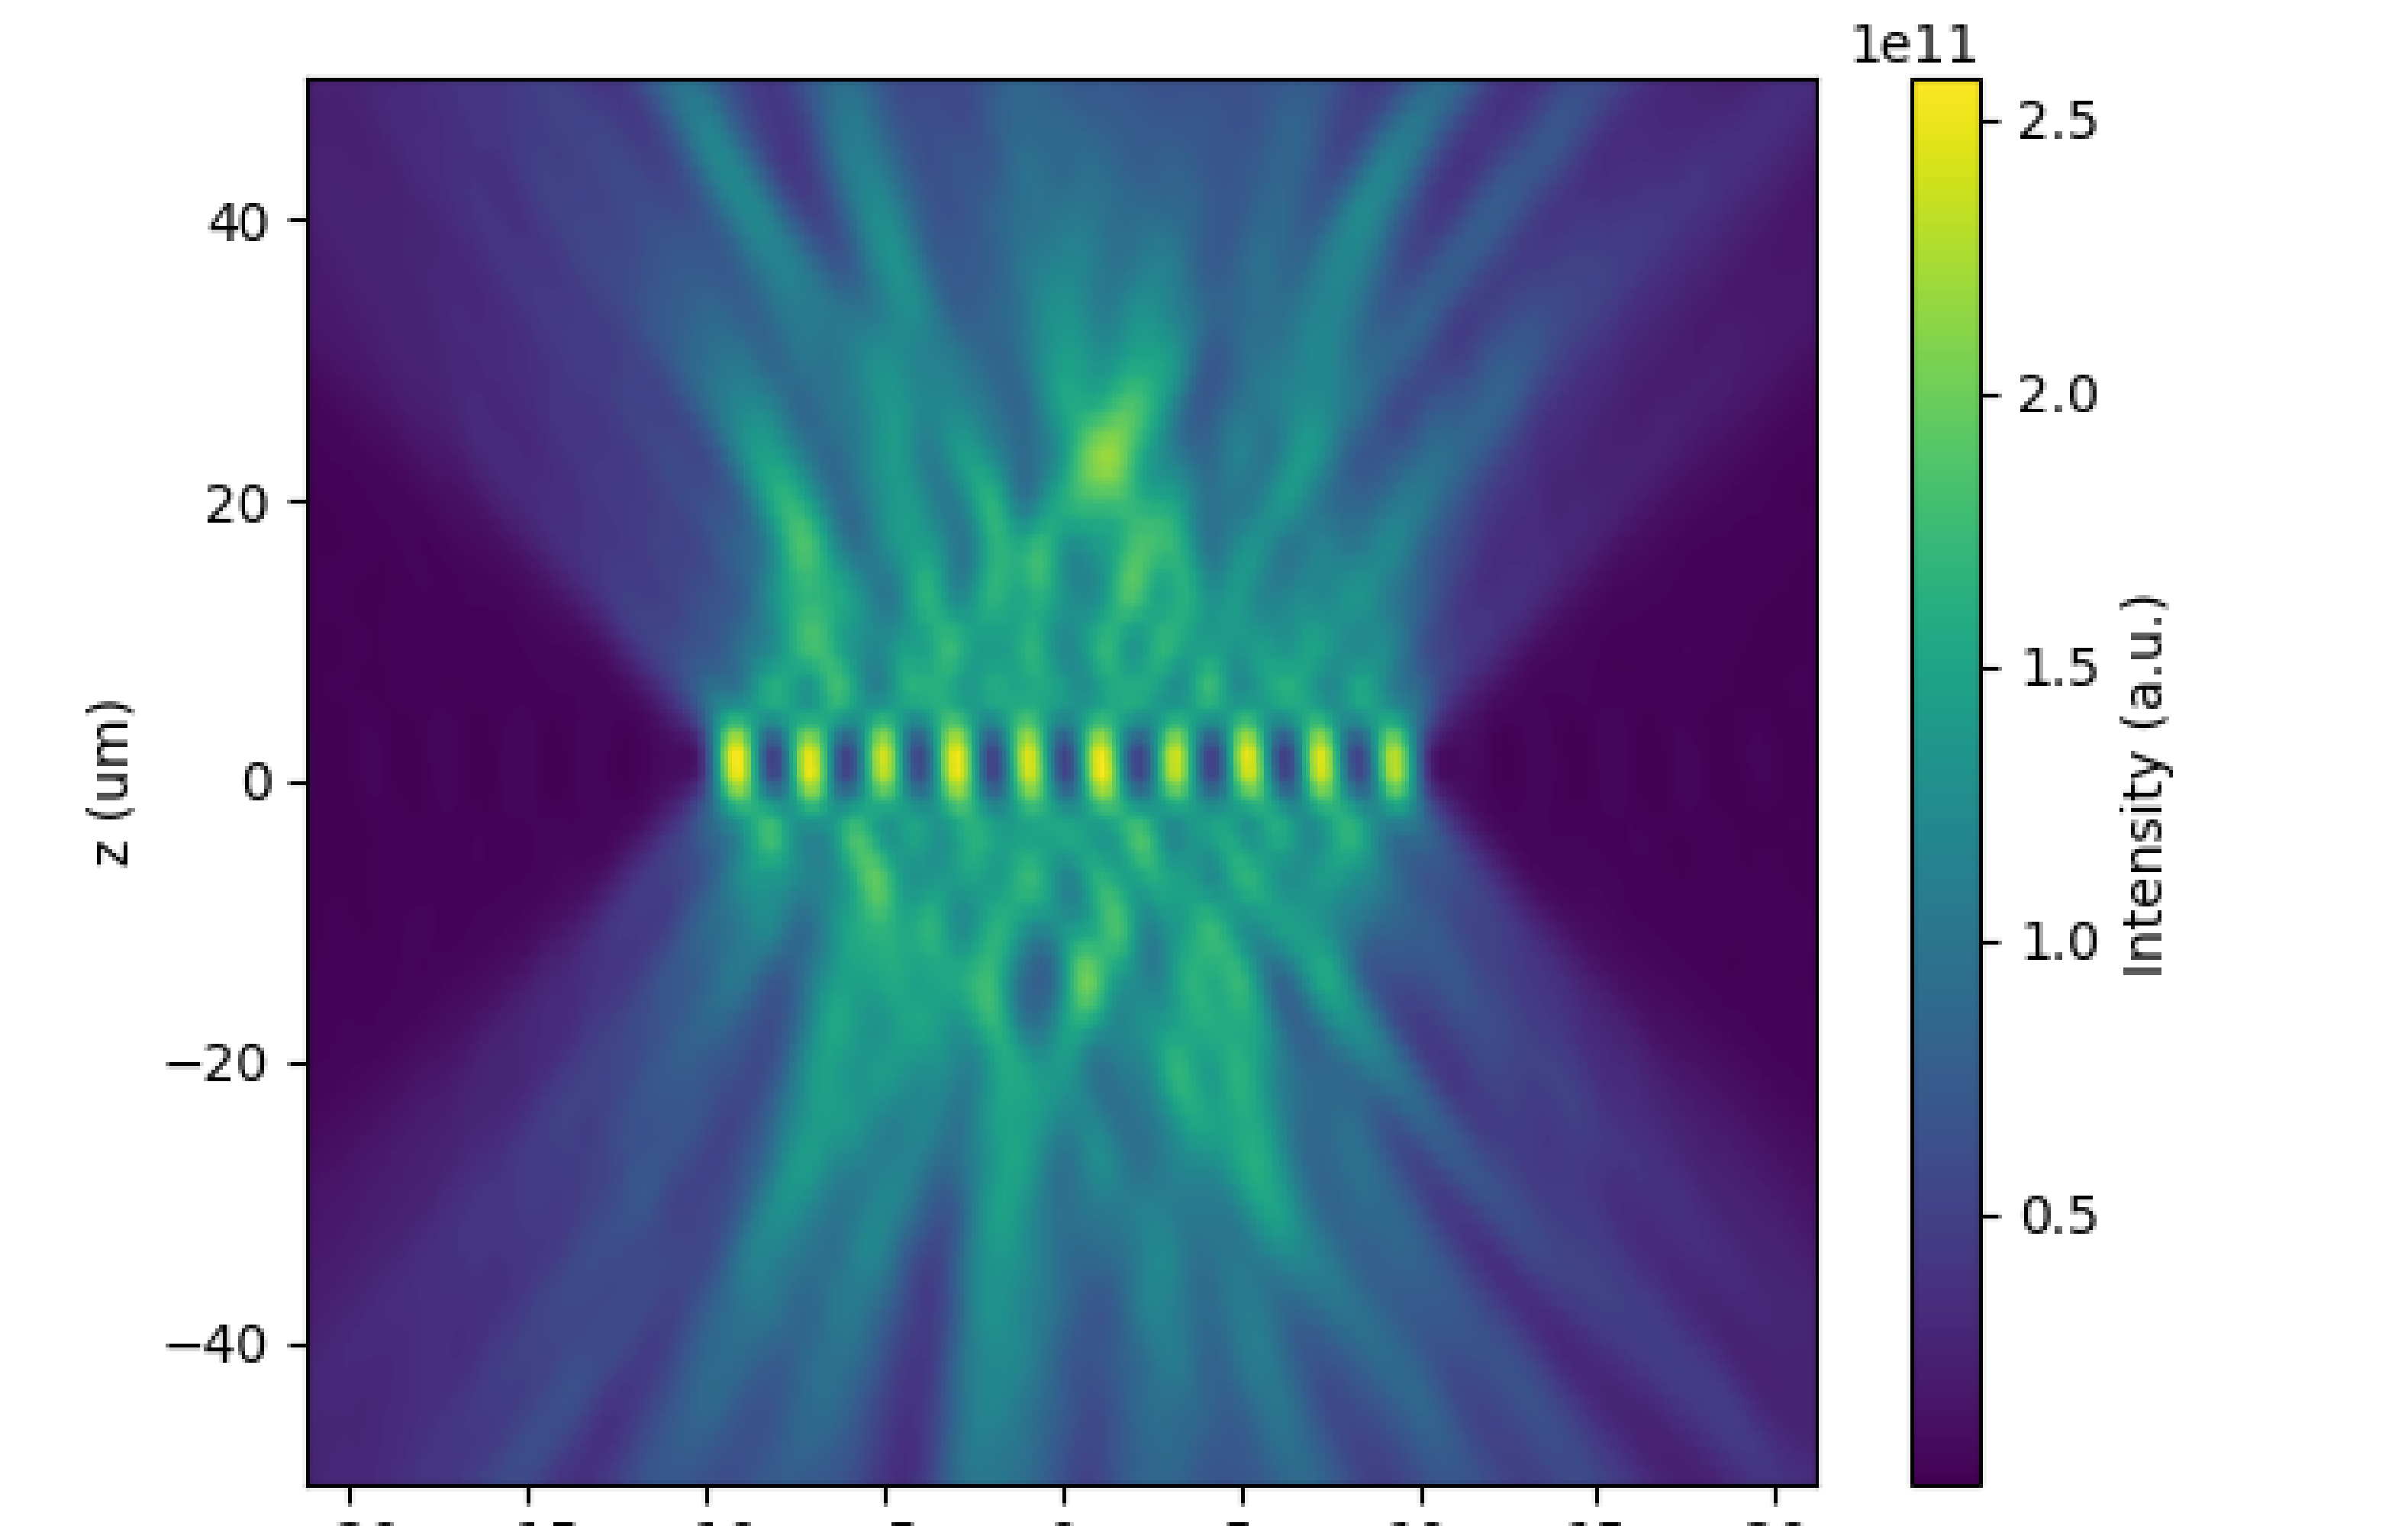
\includegraphics[height=0.65\textheight]{qsmol_figs/crop-27-lower.png}
	\hspace{1cm}
	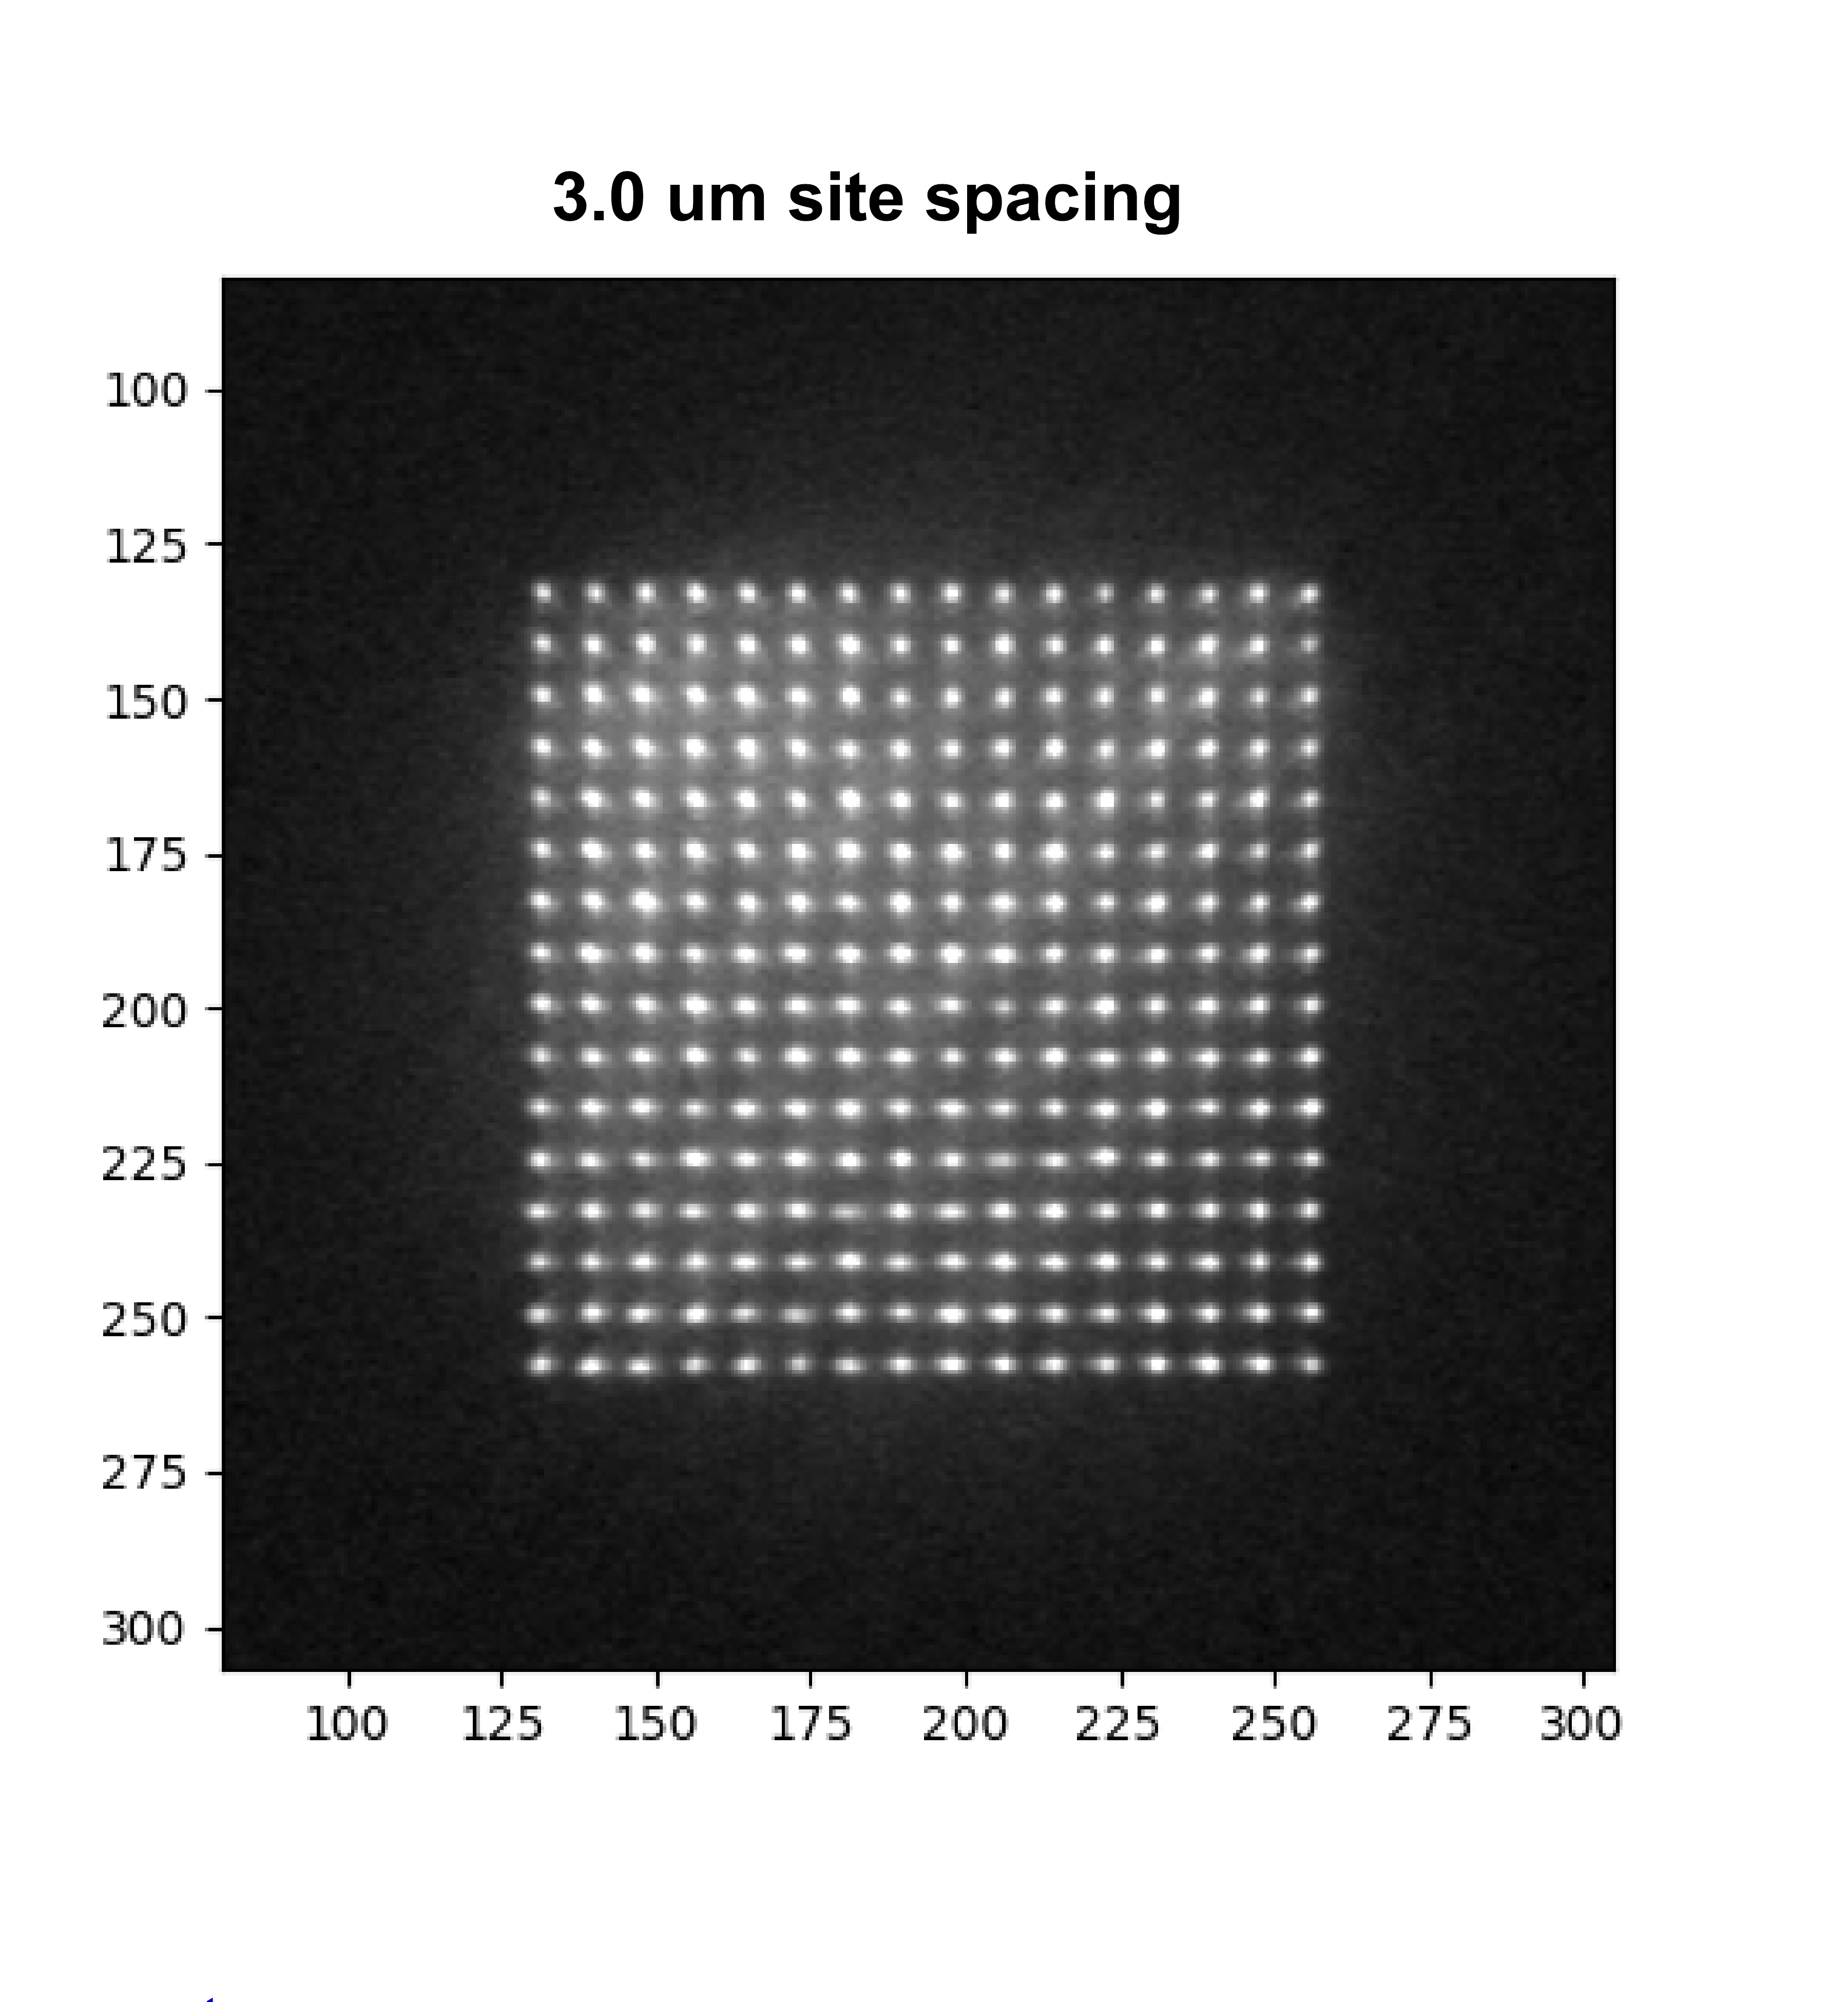
\includegraphics[height=0.75\textheight]{qsmol_figs/crop-28.png}
\end{frame}

%------------------------------------------------

\begin{frame}
	\frametitle{Dense Arrays}

	\begin{columns}[T]
		\begin{column}{0.42\linewidth}
			\small
			\textbf{For two-qubit hybrid gates need small trap site separation \textasciitilde 2.0 um for high-fidelity operations.}

			Challenges:
			\begin{itemize}
				\item Interference of tweezer light, deep off-plane traps which can efficiently trap, reduces detection fidelity.
				\item Interference between neighbouring trap sites, distorts trap potential.
				\item Rearrangement linear interpolation method breaks down for small site spacing.
			\end{itemize}
		\end{column}
		\begin{column}{0.56\linewidth}
			\centering
			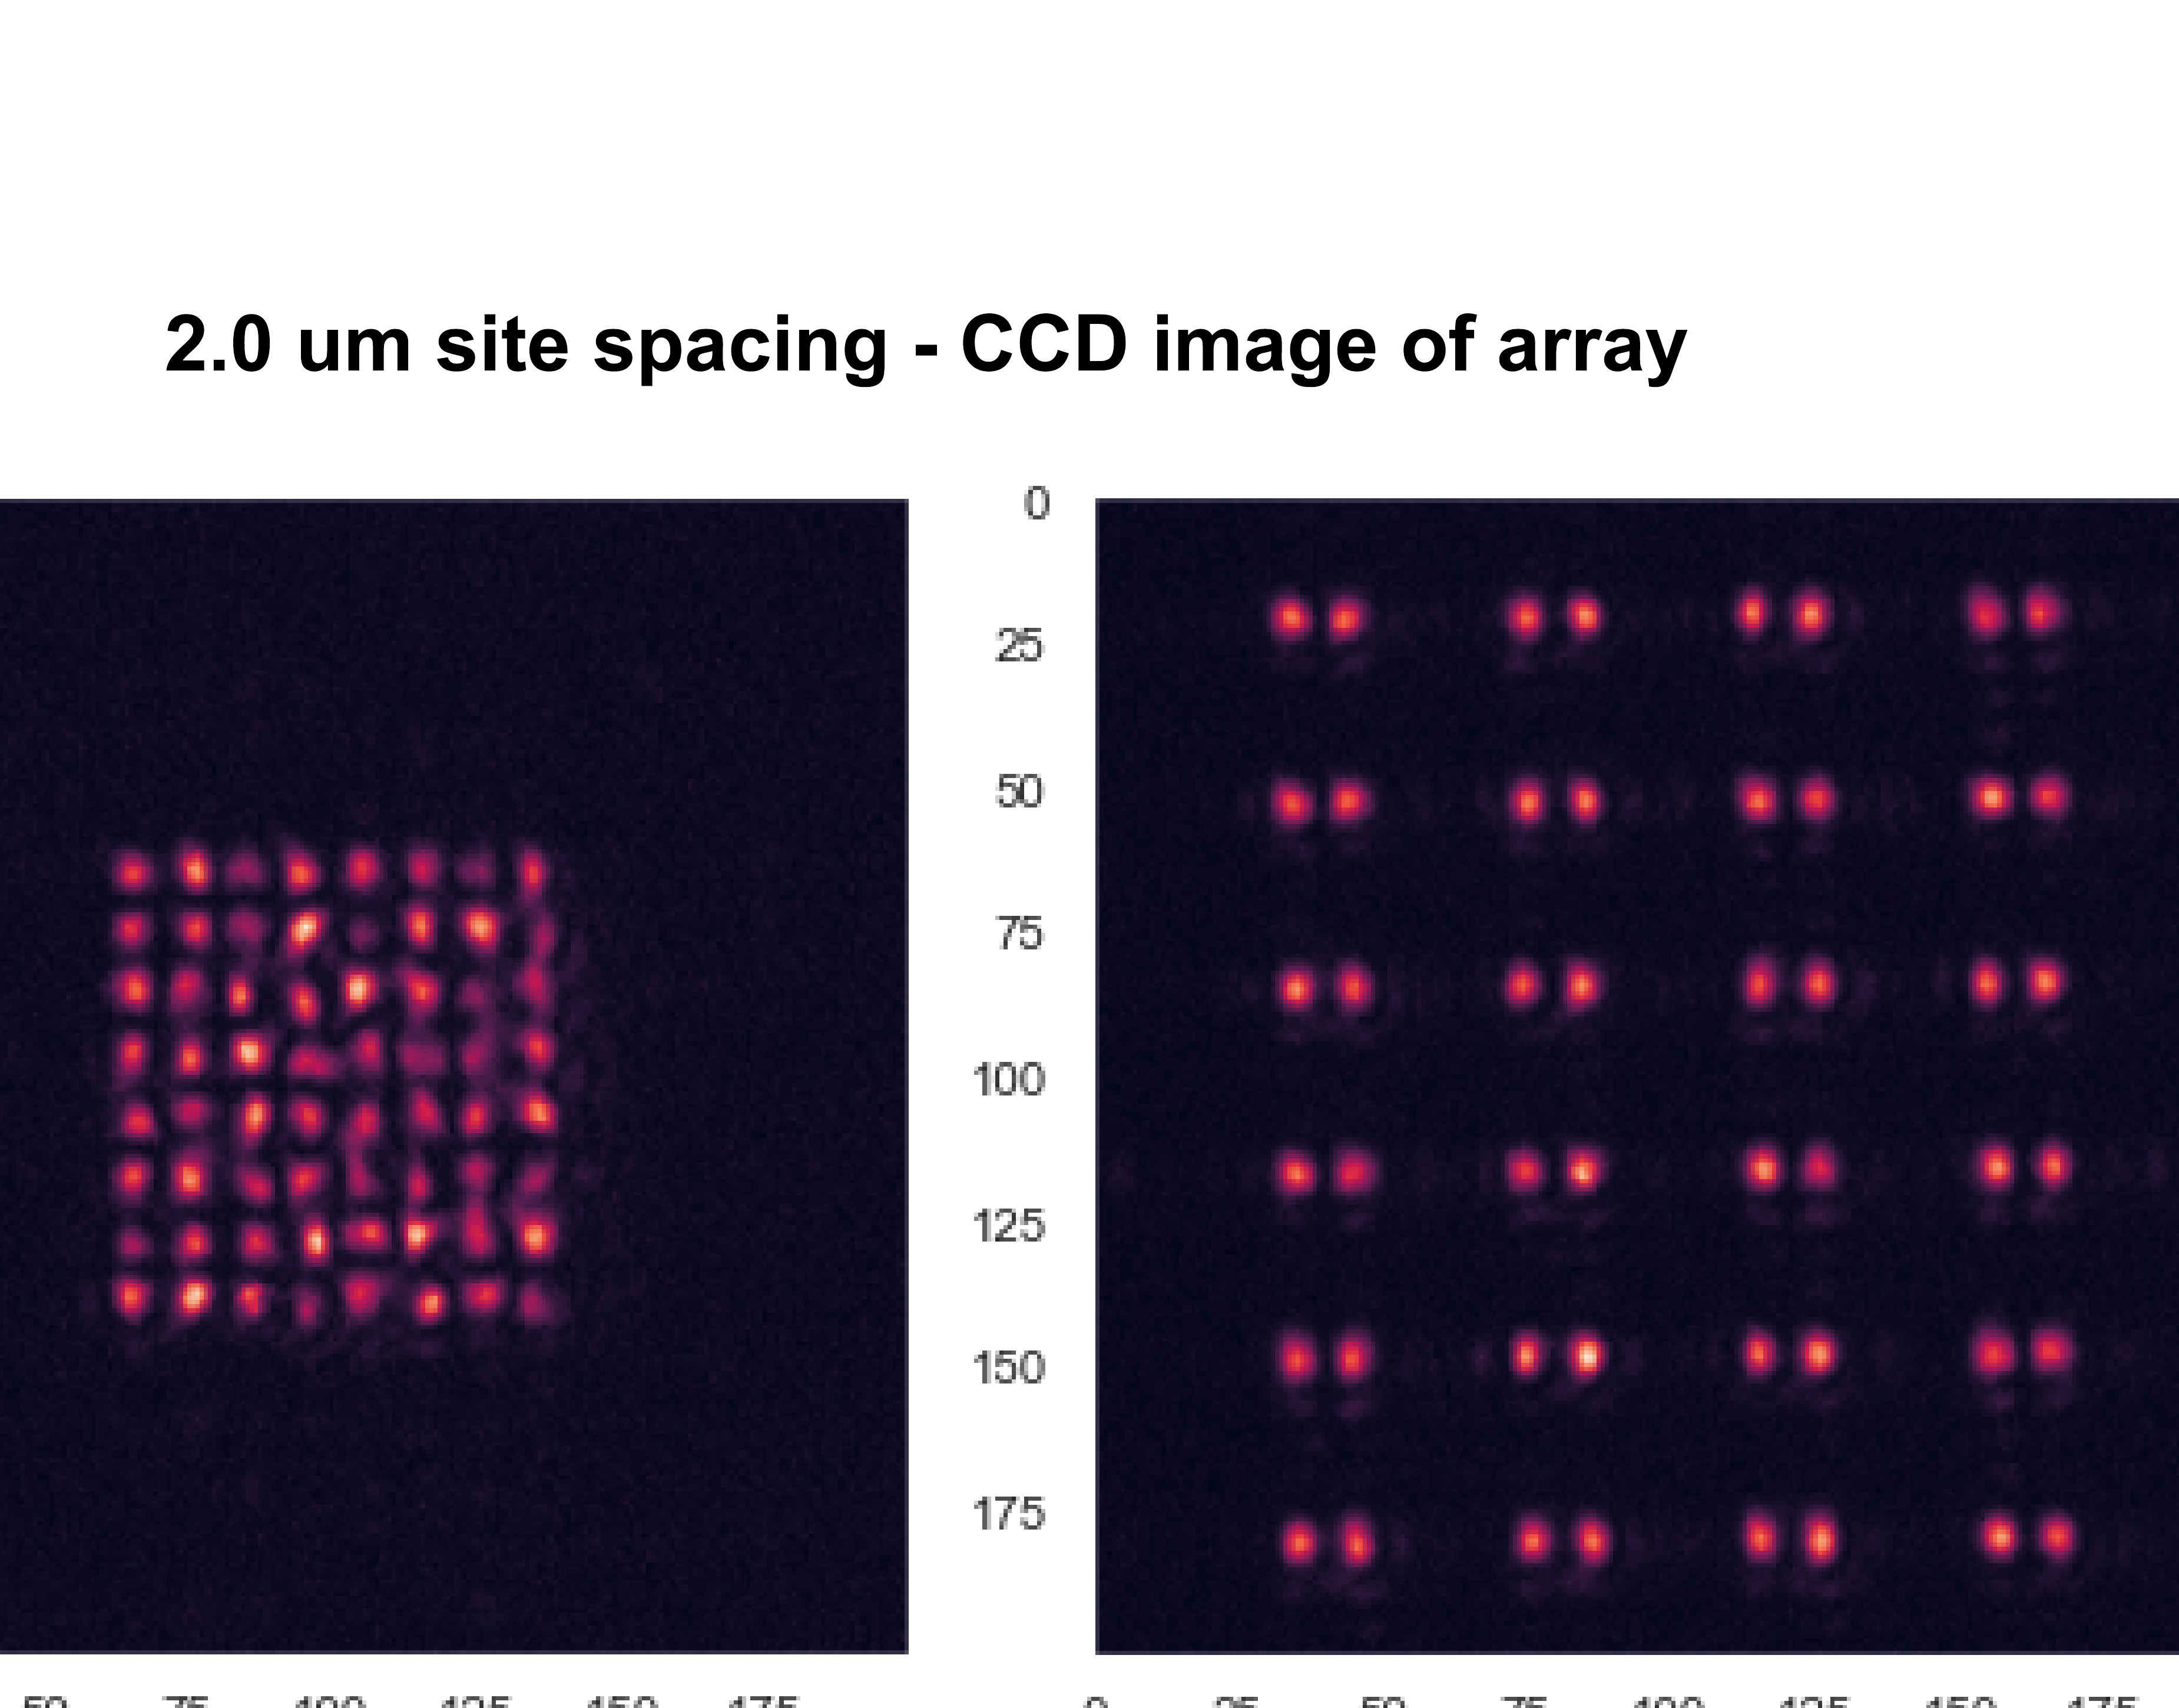
\includegraphics[width=\linewidth]{qsmol_figs/crop-29.png}
		\end{column}
	\end{columns}
\end{frame}

%----------------------------------------------------------------------------------------
%	CURRENT EFFORTS
%	(reused from the QSMol talk)
%----------------------------------------------------------------------------------------

%----------------------------------------------------------------------------------------
%	CLOSING SLIDE
%----------------------------------------------------------------------------------------

\begingroup
	\setbeamercolor{background canvas}{bg=ICLBlue}
	\setbeamercolor{normal text}{fg=white}\usebeamercolor[fg]{normal text}
	\setbeamertemplate{closing slide logo}[logo]{ICL_Logo_White.pdf}
	\setbeamertemplate{closing slide text}[text]{Thank you}

	\usebeamertemplate{closing slide}
\endgroup

%----------------------------------------------------------------------------------------

\end{document}
